\documentclass[3p, 11pt]{elsarticle}


%% Use the option review to obtain double line spacing
%% \documentclass[preprint,review,12pt]{elsarticle}

%% Use the options 1p,twocolumn; 3p; 3p,twocolumn; 5p; or 5p,twocolumn
%% for a journal layout:
%% \documentclass[final,1p,times]{elsarticle}
%% \documentclass[final,1p,times,twocolumn]{elsarticle}
%% \documentclass[final,3p,times]{elsarticle}
%% \documentclass[final,3p,times,twocolumn]{elsarticle}
%% \documentclass[final,5p,times]{elsarticle}
%% \documentclass[final,5p,times,twocolumn]{elsarticle}

%% The graphicx package provides the includegraphics command.

%\usepackage[utf8]{inputenc}
\usepackage[english]{babel}
\usepackage[T1]{fontenc}
\usepackage[utf8]{inputenc}
%\usepackage{graphicx}
\usepackage{hyperref}
\usepackage{amssymb}
\usepackage{amsmath}
\usepackage{amsthm}
\usepackage{subcaption}
\usepackage{siunitx}
\sisetup{group-separator = {,}}

\usepackage{multirow}
\usepackage{cancel}

\journal{EJOR}

%\usepackage{xcolor}
\usepackage[dvipsnames]{xcolor}

\usepackage[mathscr]{eucal}
\newcommand{\R}{\mathbb{R}}
\newcommand{\Co}{\mathbb{Co}}
\newcommand{\D}{\mathscr{D}}
\newcommand{\Pp}{\mathscr{P}}
\newcommand{\Cc}{\mathscr{C}}
\newcommand{\E}{\mathscr{E}}
\newcommand{\F}{\mathscr{F}}
\newcommand{\Ww}{\mathscr{W}}
\newcommand{\Rr}{\mathscr{R}}
\newcommand{\norm}[2][2]{\left\lVert#2\right\rVert_{#1}}
\newcommand{\bigO}{\mathscr{O}}
\newtheorem{thm}{Theorem}
\newtheorem{prp}{Proposition}
\newtheorem{lem}{Lemma}
\newdefinition{rmk}{Remark}
\newdefinition{definition}{Definition}
%\newproof{pf}{Proof}
%\renewcommand\qedsymbol{$\blacksquare$}

\bibliographystyle{elsarticle-template/model2-names}
%\biboptions{longnamesfirst,angle,semicolon}


\RequirePackage{algorithm, algpseudocode}
\renewcommand{\algorithmicrequire}{\textbf{Input:}}
\renewcommand{\algorithmicensure}{\textbf{Output:}}
\newcommand{\algorithmautorefname}{Algorithm}
\newcommand{\definitionautorefname}{Definition}
\newcommand{\thmautorefname}{Theorem}
\newcommand{\prpautorefname}{Proposition}
\newcommand{\lemmaautorefname}{Lemma}
\newcommand{\lemautorefname}{Lemma}
\newcommand{\sigla}[2]{#2 (#1)}
\newcommand{\citeonline}[1]{\cite{#1}}

\begin{document}
	
	\begin{frontmatter}
		
		%% Title, authors and addresses
		
		\title{New Exact Algorithms for Planar Maximum Covering Location by Ellipses Problems\tnoteref{t1}}
	%	\tnotetext[t1]{This paper is the results of the research
	%		project funded by CAPES and FAPESP.}
		
		\author[add1]{Danilo Tedeschi\corref{cor1}}
		\ead{danilof.t2@gmail.com}

		
		\author[add1]{Marina Andretta}
		\ead{andretta@icmc.usp.br}
					
		\address[add1]{Departamento de Matemática Aplicada e Estatística, Instituto de Ciências Matemáticas e de Computação, Universidade de São Paulo, Avenida Trabalhador São-carlense, 400, Centro, 13566-590, São Carlos, SP, Brazil.}
		
		\cortext[cor1]{Corresponding author.}
\end{frontmatter}
\clearpage
%\begin{frontmatter}
%		\begin{abstract}

\section*{Abstract}
			%% Text of abstract
			
			{\color{Red}
		Planar Maximum Covering Location by Ellipses is an optimization problem where one wants to choose the location of ellipses given their major and minor axis to cover demand points, maximizing a function depending on the value of covered points.	
		}We propose new exact algorithms for two versions of this problem, one where the ellipses have to be parallel to the coordinate axis, and another where they can be freely rotated. 
			Besides finding optimal solutions for previously published instances, including the ones where no optimal solution was known, both algorithms proposed by us were able to obtain optimal solutions for some new larger instances 	with up to seven hundred demand points and five ellipses.
\subsection*{Keywords}
			Combinatorial optimization, planar maximal covering location problem, planar covering by ellipses, exact algorithms.
			%% keywords here, in the form: keyword \sep keyword
			
			%% MSC codes here, in the form: \MSC code \sep code
			%% or \MSC[2008] code \sep code (2000 is the default)
			
%		\end{keyword}
		
%	\end{frontmatter}
	

\section{Introduction}\label{section:introduction}

\sigla{MCLP}{The Maximum Covering Location Problem}, introduced in \cite{church:1974}, is 
a problem defined on graphs where the objective is to maximize the coverage of a demand set, a subset of the graph's vertices, by choosing the location of a fixed number of facilities, with each facility covering every demand node located within a predefined radius from it. 
MCLP was introduced motivated by the practical observation that covering one hundred percent of a population, which was the subject of most of the covering location problems at that time, can take much more resources than covering ninety percent of it.

A continuous extension of MCLP, where the facility and demand sets are located on the plane and coverage is determined by a norm function, was introduced in \cite{church:1984} and named \sigla{PMCLP}{Planar Maximal Covering Location Problem} following the advances on covering location problems on the plane that were being made at the time.

{\color{Red}PMCLP can be seen as a class of problems, as, in general, facilities can have their coverage defined by any norm function, and the demand set, although initially defined as points, could have a more generic definition; in \cite{bansal}, for example, the demand set is defined as a set of rectangles; and in \cite{younies}, a version of PMCLP where coverage is determined using block norms is studied. For a more comprehensive review on PMCLP and MCLP, please see \cite{murray}.}

{\color{Red}In our work, because of the similarities with the problems studied by us, we are particularly interested in the Euclidean PMCLP defined with coverage being determined by the Euclidean norm. In \cite{church:1984}, a method for this version of PMCLP was developed following the demonstration of a theorem, which showed that a finite set of locations could be constructed to contain at least one optimal solution transforming PMCLP into a combinatorial optimization problem.} 

The Euclidean PMCLP is also found in the literature in an algorithmic context as the \sigla{MCD}{Maximum Covering by Disks Problem}.
In \citeonline{chazelle:1986}, a $\bigO(n^2)$ algorithm for the one-disk version of MCD was proposed, beating the prior $\bigO(n^2\log{n})$ algorithm created in \citeonline{drezner} for the same problem.
A version with multiple unit disks was studied in \citeonline{cabello:2006}, which had as its most important result a $(1-\epsilon)$-approximation algorithm which runs in $\bigO(n\log{n})$. To achieve its main goal, they developed a deterministic $\bigO(n^{2m-1}\log{n})$ algorithm which gets employed into their approximation scheme.
Additionally, in \citeonline{aronov:2008}, one-disk MCD is proven to be 3SUM-HARD. This means that maximizing the number of points covered by a disk is as hard as finding three real numbers that sum to zero among $n$ given real numbers.

We study two versions of PMCLP with elliptical coverage facilities in this work. For both of them, each ellipse is defined to have {\color{Red}fixed major and minor axis} and an undefined location, which is part of the solution.
In the first version, introduced in \cite{canbolat}, all the ellipses are restricted to be axis-parallel, while in the second version, introduced in \cite{andreta}, this constraint is dropped, and all the ellipses can be freely rotated.
The first version will be referred to as \sigla{MCE}{Planar Maximum Covering Location by Ellipses Problem} and the second one as  \sigla{MCER}{Planar Maximum Covering Location by Ellipses with Rotation Problem}.

%New paragraph
{\color{Orange}
	In the real world, this problem comes up when a telecommunications company has to buy and place antennas over a region to distribute a signal to a population, not necessarily everyone, aiming profit maximization. 
	More details about the applications of PMCLP can be found in \cite{canbolat}, which also ponders about the practical importance of considering the PMCLP with elliptical coverage.
	
	As a first approach to solving MCE, a mixed-integer non-linear programming method was proposed in \cite{canbolat}. 
	Its performance was measured using a constructed set of instances. The results were considered unsatisfactory, as, for some instances, the method could not find an optimal solution within an hour. 
	For this reason, a second method using a heuristic technique called Simulated Annealing was developed. For the same set of instances, the heuristic was able to obtain solutions within the predefined time limit, and for some of them, it was even able to find optimal solutions.
}

The problem was further explored in \citeonline{andreta}, where exact methods were developed for both MCE and MCER, and a heuristic method was developed for MCER.
All the methods proposed in \cite{andreta} were based on the enumerative approach of solving optimization subproblems to determine whether an ellipse could cover a subset of demand points or not. To avoid having to solve subproblems for every subset of demand points, a tree-like data structure was designed to skip non-maximal sets of demand points.
The only difference in their methods for MCE and MCER was the subproblem.
As the subproblem for MCE was a convenient convex optimization model, the method for it performed well and  was able to obtain optimal solutions for instances the method from \cite{canbolat} could not.
The subproblem for MCER, on the other hand, was more challenging, and ended up making the method time out for large instances. For this reason, a heuristic method was developed treating the optimization subproblem as a convex problem. The method was able to obtain solutions for every instance, and for the ones the exact method did not time out, it could be verified that the heuristic method returned optimal {\color{blue}solutions} as well.

Based on the developments of \cite{church:1984} for the Euclidean PMCLP, we define a finite set of solutions for each one of the problems, MCE and MCER, which we prove to contain at least one optimal solution, and that, if the number of facilities is assumed to be constant, its size is bounded by a polynomial.
We propose algorithms for both problems based on the computation of this set of solutions to determine an optimal one.
For MCER, computing this set of solutions involves solving a subproblem, on which we could not find any prior study, thus, a whole section is devoted to the development of an algorithm for it.
Besides all that, we give implementation details for both algorithms, and also improvement suggestions which, in practice, can significantly lower the number of solutions evaluated to return an optimal one.
In the end, we analyze numerical experiments for instances proposed in \cite{canbolat, andreta} and compare the results with the results obtained by the methods proposed in \cite{andreta}. Also, to further {\color{blue}evaluate} our algorithms, we analyzed numerical experiments for new instances with larger demand and facility sets.

{\color{Red}
This paper is organized as follows. Section~\ref{section:definition} presents the definitions of both problems and introduces some notations used throughout the rest of the work. An algorithm for MCE is developed in Section~\ref{section:mce}, and an algorithm for MCER in Section~\ref{section:mcer} with the observation that its development depends on a subproblem whose algorithm is developed in Section~\ref{section:e3p}. Improvements suggestions to the implementations are given in Section~\ref{section:improvements} while the implementation details are given in Section~\ref{section:implementation}. Numerical results are presented and analyzed in Section~\ref{section:numerical}. Finally, a conclusion is given in Section~\ref{section:conclusion}.
}

\section{Definition}\label{section:definition}
%Given $n$ demand points $\Pp:=\{p_1, \dots, p_n\}$, with weights $\Ww:=\{w_1, \dots, w_n\}$, $w_i\in\R_{\ge0}$; and $m$ shape parameters $\Rr:=\{(a_1, b_1); \dots; (a_m, b_m)\}$, with $(a_j, b_j) \in \R_{>0}^2$ being the semi-major and semi-minor axis of the $j$-th ellipse. 

%For MCE, $\Rr$ describes the shape parameters of $m$ axis-parallel ellipses, and we want to determine a center $q_j\in\R^2$ for each one of them to maximize the weight of the covered points. For MCER, $\Rr$ describes the shape parameters of ellipses that not necessarily are axis-parallel, and we want to determine a center $q_j \in \R^2$, and an angle of rotation $\theta_j\in[0, \pi)$ for each ellipse to maximize the weight of the covered points. 


An instance of MCE and MCER is given by $n$ distinct demand points $\Pp=\{p_1, \dots, p_n\}$, $p_j\in\R^2$; $n$ weights $\Ww=\{w_1, \dots, w_n\}$, with $w_j\in\R_{>0}$ being the weight of the $j$-th point; and $m$ shape parameters $\Rr=\{(a_1, b_1), \dots, (a_m, b_m)\}$, with $(a_j, b_j)\in\R_{\ge0}^2$ being the semi-major and semi-minor axis of the $j$-th ellipse, with $a_j > b_j > 0$.

For MCE, the shape parameters describe axis-parallel ellipses, and the problem is to determine a center for each ellipse to maximize the weight of covered demand points. For MCER, besides the center, because the ellipses are not necessarily axis-parallel, for each facility, an angle of rotation is also part of the solution, and the problem is to maximize the weight of covered demand points as well.

Let $\E=\{E_1, \dots, E_m\}$ be a list of functions representing the coverage area of each facility, with $E_j \colon \R^2 \to \R^2$ for MCE, and $E_j \colon \R^2\times [0, \pi)\to \R^2$. Let $||\cdot||_{a,b, \theta} \colon \R^2 \to \R_{\ge0}$ denote the elliptical norm given by
\begin{equation*}
||x||_{a,b, \theta}=\left|\left|
\left(\begin{array}{rr}
\cos{\theta} & \sin{\theta}\\
\sin{\theta} & -\cos{\theta}
\end{array}
\right)
\left(\begin{array}{cc}
a_j & 0\\
0 & b_j
\end{array}\right) x \right|\right|_2,
\end{equation*}
then, for MCE we define $E_j(q)=\{p \in \R^2 \colon ||p-q||_{a_j,b_j,0} \le 1\}$; and for MCER we define $E_j(q, \theta)=\{p \in \R^2 \colon ||p-q||_{a_j,b_j, \theta} \le 1\}$.

To make the notation more clear, we define a solution of MCE as $Q:=(q_1, \dots, q_m)$, and a solution of MCER as $Q:=((q_1, \theta_1); \dots; (q_m, \theta_m))$. 
Let $w : A \subset \Pp \to \R$ be a function which takes a subset of the demand set and returns the sum of the weights of the points in $A$. Then, we define MCE  as the optimization problem 
\begin{equation*}
\max_{Q}  w\left(\cup_{j=1}^m\Pp \cap E_j(q_j)\right),
\end{equation*}
and similarly MCER as
\begin{equation*}
\max_{Q} w\left(\cup_{j=1}^m\Pp \cap E_j(q_j, \theta_j)\right).
\end{equation*}

We define an equivalence and a partial order relation between solutions of both MCE and MCER as follows.
Two solutions $Q$ and $Q'$ of MCE (MCER), are said to be equivalent to each other if
they both cover the same set of demand points.
% $\cup_{j=1}^m \Pp \cap E_j(q_j) = \cup_{j=1}^m \Pp \cap E_j(q_j')$ ($ \cup_{j=1}^m \Pp \cap E_j(q_j, \theta_j) = \cup_{j=1}^m \Pp \cap E_j(q_j', \theta_j')$). That is, two solutions are equivalent if they cover the same set of points.
We also define a partial order: $Q' \succ Q$ if, and only if the set of demand points covered in solution $Q$ is a subset of the demand points covered in solution $Q'$.

%if, and only if $\cup_{j=1}^m \Pp \cap E_j(q_j) \subset \cup_{j=1}^m \Pp \cap E_j(q_j')$ ($\Pp \cap\cup_{j=1}^m E_j(q_j, \theta_j) \subset \Pp \cap\cup_{j=1}^m E_j(q_j', \theta_j')$). That is, $Q' \succ Q$ if, and only if the set of points covered in solution $Q$ is a subset of the points covered in solution $Q'$.

%%% esse paragrafo ainda ta estranho.
Additionally, we denote by $\partial$ the boundary operator, for example, given an instance of MCE, $\partial E_1(q_1)$ represents the set of points $\{p \in \R^2\colon ||p-q_1||_{a_1,b_1,0} = 1\}$. Also, whenever we have an instance $(\Pp, \Ww, \{(a, b)\})$ with only one facility, we omit the index referring to the ellipse. 

\subsection{Facility Cost}

In \cite{canbolat, andreta}, as a result of having costs assigned to each facility, two other parameters are present in the definition of the problem.
These new parameters are: the list of costs $\Cc=\{c_1, \dots, c_m\}$, with $c_j\in\R_{\ge0}$ being the $j$-th ellipse's cost; 
and an integer $k\in\mathbb{N}$, $k\le m$, which introduces a constraint requiring that exactly $k$ facilities have to be utilized.
Because of that, a solution also needs an additional parameter $I:=\{i_1, \dots, i_k\}\subset\{1, \dots, m\}$ to express the indexes of the utilized ellipses. We refer to this version of the problem as  MCE-$k$ and MCER-$k$.

From an algorithm for MCE (MCER), we can propose an algorithm for MCE-$k$ (MCER-$k$), which just takes the best overall solution among the $\binom{m}{k}$ instances $(\Pp, \Ww, \Rr')$, such that $\Rr' \subset \Rr$ and $|\Rr'| = k$. 
Therefore, in our work, we focus on developing algorithms for MCE and MCER, and whenever we refer to an algorithm for MCE-$k$ (MCER-$k$), we mean an algorithm as described here, which considers all the $\binom{m}{k}$ instances of MCE (MCER).


%Therefore, as this step can be seen as trivial, we focus on proposing algorithms for MCE and MCER, and in the section where we analyze the numerical experiments, as we use instances from \cite{andreta}, whenever we refer to an algorithm of MCE-$k$ (MCER-$k$), see it as an algorithm based on the approach described here, which uses $\binom{m}{k}$ instances of MCE (MCER) to obtain an optimal solution.

\section{An Algorithm for MCE}\label{section:mce}

In this chapter, we introduce the version of PMCLP where every 
facility has an axis-parallel ellipse as its coverage area. We refer to this problem as \sigla{MCE}{Maximum Covering by Ellipses}. We also present an algorithm for it which is an adaptation of the algorithm developed for MCD in \autoref{chapter:pmclp}.

\section{Definition}

Axis-parallel ellipses are defined as the set of points that satisfy \autoref{equation:pellipse}. Note that all it takes to describe an axis-parallel ellipse is a pair of positive real numbers $(a,b) \in \R_{>0}^2$, also called its shape parameters, and a center point $q \in \R^2$.

An instance of MCE is given by a set of $n$ demand points $\Pp = \{p_1, \dots, p_n\}$, with $p_j\in\R^2$; 
a set of weights $\Ww:=\{w_1, \dots, w_n\}$, with $w_j\in\R_{\ge0}$ being the weight of point $p_j$;
and a set of $m$ axis-parallel ellipses given by their shape parameters $\Rr:=\{(a_1, b_1), \dots, (a_m, b_m)\}$, with $(a_j, b_j)\in\R_{>0}^2$ and $a_j>b_j$.
Additionally, to make the text more clear, we define a set $\E = \{E_1, \dots, E_m\}$, with $E_j : \R^2 \mapsto \R^2$ being a function that takes the center where the $j$-th ellipse is located as input, and returns its coverage region as defined by \autoref{equation:cover_pellipse}.

Then, a solution for MCE is given by $Q:=(q_1, \dots, q_m)\in\R^{2m}$, with $q_j$ being the center of $j$-th ellipse. Finally, let $w : 2^\Pp \mapsto \R_{\ge0}$ as defined by \autoref{eq:subset_w}, then an optimal solution of MCE is given by the optimization problem

\begin{equation*}
\max_q w\left(\bigcup_{j=1}^m \Pp \cap E_j(q_j)\right).
\end{equation*}

In the next sections, we first describe a method for the case with only one ellipse, and then use it in the algorithm for multiple ellipses to construct a CLS containing an optimal solution.

\section{Related work}
The maximal planar covering using axis-parallel ellipses was first introduced in \citeonline{canbolat} which proposed a mixed integer non-linear programming method for the problem. This first approach showed to be not that efficient as it could not find an optimal solution for some instances within a timeout defined by them. To obtain solutions, not necessarily optimal ones, for the instances which the exact method showed inefficiency, a heuristic technique called Simulated Annealing was used to develop another method. Comparisons were made, which showed that the second approach was able to obtain good solutions, compared to the optimal ones found for some of the instances, within a good run-time.

The second work found in the literature was \citeonline{andreta}, which developed a method that breaks the problem into smaller ones fixing the set of points an ellipse is going to cover. For each set of points fixed as the points an ellipse is going to cover, a small optimization problem is solved to find out if there is a location where the ellipse can be placed, so to cover the set of fixed points. To enumerate the possible solutions and then find an optimal one, the method defined a data structure that stores every set of points an ellipse can cover. This method showed better results and was able to find optimal solutions for the instances that the first method could not get as well as for new created instances.

\section{One Ellipse Version}

The case with only one ellipse is considered first because it will be adapted to become the basis of the algorithm for more than one ellipse. We refer to this version as \sigla{MCE-1}{Maximum Cover by One Ellipse}. 

An instance of MCE-1 has $m=1$, and we set $(a, b):=(a_1, b_1)$, and $\E := \{E\}$. Therefore, an instance of MCE-1 is described by the tuple $(\Pp; \Ww; (a, b))$. A solution of MCE-1 is then given by a point $q\in\R^2$, and an optimal solution is given by the optimization problem

\begin{equation*}
\max_q w(\Pp \cap E(q)).
\end{equation*}
An adaptation of \autoref{algoritmo:mcd_1} is obtained by just replacing the function that finds the intersection points between two disks by a function that finds the intersection points between two ellipses $\partial E_i$ and $\partial E_j$.
It can be seen in \autoref{fig:3ellipses_intersect} that the intersection points and their correspondents $\Gamma_-(i,j)$ and $\Gamma_+(i,j)$ functions behave the same way as in the disks case.
The intersection of two ellipses as well as determining $\Gamma_-(i,j)$ and $\Gamma_+(i,j)$ are described in the next section.

\begin{figure}[H]
	\centering
	\caption{Three ellipses and their intersection points}
	\includegraphics[scale=.34]{tex/figures/3ellipses_intersect.pdf}
	\fautor
	\label{fig:3ellipses_intersect}
\end{figure}

\section{Determining $\Gamma_+(i,j)$ and $\Gamma_-(i,j)$}\label{section:ellipses_intersection}

Let $E_1(q_1)$, and $E_2(q_2)$ be two coverage region of ellipses centered at $q_1, q_2\in\R^2$ respectively, with shape parameters $(a, b)\in\R^2_{>0}$. After changing the coordinates to make the center of the first ellipse be at the origin, the intersection points between the two ellipses are defined by

\begin{align}
\frac{x^2}{a^2} + \frac{y^2}{b^2} = 1 && (E_1) \label{eq:ell_inter_1}\\
\frac{(x-h)^2}{a^2} + \frac{(y-k)^2}{b^2} = 1 && (E_2), \nonumber
\end{align}
where $(h,k)\in\R^2$ is the center of the second ellipse after the coordinates were translated by $-q_1$. As both equations are equal to $1$, we have
\begin{align}
    b^2x^2 + a^2y^2 &= b^2(x-h)^2 + a^2(y-k)^2 \nonumber\\
    x &= y\frac{-2ka^2}{2hb^2} + \frac{b^2h^2 + a^2k^2}{2hb^2} \nonumber\\
    x &= y\alpha + \beta.\label{eq:ell_inter_2}
\end{align}
Replacing \autoref{eq:ell_inter_2} into \autoref{eq:ell_inter_1}, we get
\begin{align}\label{eq:ell_inter_3}
y^2(b^2\alpha^2 + a^2) + y(2\beta\alpha b^2) + b^2\beta^2 -a^2b^2 = 0,
\end{align}
Which is a second degree polynomial. Then, $\partial E_1(q_1) \cap \partial E_2(q_2) \neq \{\}$ if, and only if the roots of \autoref{eq:ell_inter_3} are real. The intersection points itself can be obtained by solving the polynomial for $y$ and applying its value onto the $x=y\alpha + \beta$ equation.

Suppose that $\partial E_1(q_1) \cap \partial E_2(q_2) = \{p_1, p_2\}$, with $p_1 \neq p_2$. To determine $\Gamma_+(1,2)$ and $\Gamma_-(1,2)$, we need to first determine the angles of intersection of $p_1$ and $p_2$ on $E_1(q_1)$ using the parametric equation for an ellipse defined in \autoref{eq:parametric_ellipse}. Given a point $(x, y)\in \partial E_1(q_1)$, using \autoref{eq:parametric_ellipse} we have

\begin{equation*}
\dfrac{a}{b}\dfrac{y-q_{1y}}{x-q_{1x}} = \tan{t}.
\end{equation*}
Solving for $t$ gives the angle of point $(x,y)$ on $E_1(q_1)$. Using that process we obtain $t^{(1)}_1, t^{(1)}_2$ as the angles of the points $\{p_1, p_2\}$ on $E_1(q_1)$; and $t^{(2)}_1, t^{(2)}_2$ as the angles of points $\{p_1, p_2\}$ on $E_2(q_2)$.
Let $\gamma_1$ be the curve defined by $E_1(q_1)$ and $\gamma_2$ the curve defined by $E_2(q_2)$. Considering its derivatives \autoref{eq:der_parametric_ellipse} at the intersection points, as it can be seen in \autoref{fig:ellipse_gamma}, we have that $p_1$ is $\Gamma_+(1,2)$ if, and only if
\begin{equation*}
angle(\gamma_1'(t_1^{(1)}), -\gamma_2'(t_1^{(2)}) < \pi.
\end{equation*}
The case where that angle is equal to $\pi$ happens when both ellipses intersect at only one point. This case has to be treated separately as we need to have two equal intersection points: one as $\Gamma_+(1,2)$ and the other as $\Gamma_-(1,2)$.

\begin{figure}
	\centering
	
	\caption{The intersection list of a disk with three other disks.}
	%\input{tex/figures/array_disks.tex}
	\includegraphics[scale=.38]{tex/figures/ellipse_gamma.pdf}
	\fautor
	\label{fig:ellipse_gamma}
\end{figure}

\section{An algorithm for MCE}

The same procedure defined in \autoref{algoritmo:mcd_cls} can be used to get a CLS for every ellipse in MCE. We refer to the elliptical version of that procedure as CLS-MCE (we do not define it in this chapter because it would look the same as CLS-MCD defined in \autoref{algoritmo:mcd_cls}, apart from the name, of course). 

Then, with the algorithm to construct a CLS for every ellipse in hands, an algorithm for MCE naturally comes into existence. In \autoref{algoritmo:mce}, a complete search is done backtracking every possibility in the CLS of every ellipse. This strategy is backed-up by \autoref{lema:mcd}, which says that there is an optimal solution in the CLS of each ellipse. 
Following this, counting every possibility that the algorithm goes through, we arrive at the run-time complexity of $\bigO(n^{2m})$.

It is worth mentioning that, even though we call CLS-MCE every time in the recursion, in practice, it is probably best to pre-process this step, and only call it $m$ times for the whole set of points.
Some other easy improvements can also be made in the implementation. For example, if an ellipse covers two sets of points $X$ and $Y$, with $X \subset Y$, then set $X$ can be ignored by the algorithm because of the non-negative weights constraint. Also, if two ellipses have their centers with Euclidean distance greater than their semi-major parameter, they for sure do not intersect. Depending on the input, this observation can make the algorithm not go through the whole list of ellipses every time it needs to determine the ellipses pairwise intersections.

\section{Adding facility cost}

Additionally, in \citeonline{andreta} and \citeonline{canbolat}, two other parameters are present in the definition of the problem. This extension is the result of having costs associated with every facility.
In MCE, though, the total cost, which is the sum of costs of every used facility, is constant; hence, to create a decision about which ones are utilized, a new parameter $k\in\mathbb{N}$ is given, along with a constraint on the number of used ellipses.

We refer to this version of the problem as  \sigla{MCE-$k$}{Maximum Covering by Ellipses with a $k$-constraint}. An instance of it is given by the same parameters as MCE, plus a list of costs $\Cc=\{c_1, \dots, c_m\}$, with $c_j\in\R_{\ge0}$ being the $j$-th ellipse's cost, and $k\in\mathbb{N}$, $k\le m$.

 A solution for MCE-$k$, however,  when compared to MCE's, has a bit more cluttered description. We define it as a set $I:=\{i_1, \dots, i_k\}\subset\{1, \dots, m\}$, such that $|I|=k$; and a tuple $Q:=(q_1, \dots, q_k)$, with $q_j\in\R^2$ being the center of the $j$-th ellipse in $I$. An optimal solution of MCE-$k$ is given by the optimization problem

\begin{equation*}
\max_{I, Q} w\left(\bigcup_{j=1}^k \Pp \cap E_{i_j}(q_j)\right).
\end{equation*}

Finally, \autoref{algoritmo:mce} can serve as basis for the \autoref{algoritmo:mce-k} for MCE-$k$. 
Firstly, for every subset $I \subset \{1, \dots, m\}$, such that $|I| = k$, the algorithm for MCE is invoked for the instance $(\Pp, \Ww, \{(a_j, b_j) : j \in I\})$; that is, an instance where only the ellipses in $I$ are present.
After that, by keeping track of the utilized ellipses' costs for every $I \subset \{1, \dots, m\}$, an optimal solution can be obtained.
This simple adjustment achieves a run-time complexity of $\bigO(\binom{m}{k} \times n^{2k}) = \bigO(n^{3m})$. 

\begin{algoritmo}
    \caption{Algorithm for MCE}\label{algoritmo:mce}
    
    \begin{algorithmic}[1]
        \Require{A set of points $\Pp=\{p_1,\dots,p_n\}$, a list of weights $\Ww=\{w_1, \dots, w_n\}$, and a list of shape parameters $\Rr=\{(a_1, b_1), \dots, (a_m, b_m)\}$.}
        
        \Ensure{An optimal solution for MCE.}
        
        \item[]
        \Procedure{$MCE$}{$\Pp, \Ww, \Rr$}
	    \State \Return $MCE_{bt}(\Pp, \Ww, \Rr, 1)$
        \EndProcedure
        
        \Procedure{$MCE_{bt}$}{$Z, \Ww, \Rr, j=1$}
        \If{$j = m+1$}
        \State \Return $0$
        \EndIf
        
        \State $(q_j^*, \dots, q_m^*) \gets (0, \dots, 0)$

        \State $S_j \gets \textnormal{CLS-MCE}(Z, a_j, b_j)$
        \For{$q_j \in S_j$}
        \State $Cov \gets \Pp \cap E_j(q_j)$
        \State $(q_{j+1}, \dots, q_m) \gets MCE_{bt}(Z \setminus Cov, \Ww, \Rr, j+1)\}$
        
        \If{$w(Cov) + w(\cup_{k=j+1}^m Z \cap E_k(q_k)) >  w(\cup_{k=j}^m Z \cap E_k(q_k^*))$}
        \State $(q_j^*, \dots, q_j^*) \gets(q_j, \dots, q_m)$
        \EndIf
        \EndFor

        \State \Return $(q_j^*, \dots, q_m^*)$
        \EndProcedure
    \end{algorithmic}
\end{algoritmo}

\begin{algoritmo}
	\caption{Algorithm for MCE-$k$}\label{algoritmo:mce-k}

	
	\begin{algorithmic}[1]
   \Require{A set of points $\Pp=\{p_1,\dots,p_n\}$, a list of weights $\Ww=\{w_1, \dots, w_n\}$, a list of shape parameters $\Rr=\{(a_1, b_1), \dots, (a_m, b_m)\}$, a list of costs $\Cc=\{c_1, \dots, c_m\}$, and $k\in \mathbb{N}$.}
	\Ensure{An optimal solution for MCE-$k$.}
	        
	\item[]
	
\Procedure{MCE-$k$}{$\Pp, \Ww, \Rr, \Cc, k$}
	\State $I^* = \{i_1^*, \dots, i_k^*\}\gets \{1, \dots, k\}$
	\State $Q^* = (q_1^*, \dots, q_k^*) \gets (0, \dots, 0)$
	
	\ForAll{$I=\{i_1, \dots, i_k\} \subset \{1, \dots, m\}$, such that $|I|=k$}

		\State $(q_1, \dots, q_k) \gets MCE(\Pp, \Ww, \{(a_j, b_j) \in \Rr: j \in I\})$
		
			
		\If{$w(\bigcup_{j=1}^k \Pp \cap E_{i_j}(q_j)) - \sum_{j\in I} c_j > w(\bigcup_{j=1}^k \Pp \cap E_{i_j^*}(q_j^*)) - \sum_{j\in I^*}c_{j}$}
			\State $Q^* \gets (q_1, \dots, q_k)$
			\State $I^* \gets I$
		\EndIf
	\EndFor
	
	\State \Return $I^*, Q^*$
\EndProcedure
	\end{algorithmic}
\end{algoritmo}

\section{Determining Every Center and Angle of Rotation of An Ellipse Given {\color{Red} Its Shape Parameters} and Three Points that It Must Contain}\label{section:e3p}
	
The problem of finding every center and angle of rotation of a fixed shape ellipse which makes it have three points on its border is presented in this section. Even though its simple statement--it is short and uses only basic mathematical concepts--we were not able to find any work on it, or even on related problems. 
As a result, starting from scratch, we ended up trying a handful of approaches with most of them failing on the way. We try to give a review of some of those, and also make a case for the method we propose in terms of velocity of convergence and quality of the solutions that it finds.

We refer to this problem as \sigla{E3PNT}{Ellipse by Three points}, and an instance of it is given by three points $u, v, w \in \R^2$ and $E$, an ellipse with shape parameters $(a, b) \in \R^2_{>0}$, with $a > b$. A solution of E3PNT is a pair $(q, \theta) \in \R^2\times[0, \pi]$, such that $\{u, v, w\} \subset \tilde{E}(q, \theta)$. In other words, the goal is to develop a method to find every solution of E3PNT. 


\section{Transforming the problem}

To make it simpler, let us translate the system, so the point $u$ is at $(0,0)$. Then, we assume that the ellipse is actually axis-parallel and the points are the ones rotating. When an angle is found such that the three points lie on the border of the axis-parallel ellipse, a linear transformation can be applied to compress the x-axis by $\frac{b}{a}$, transforming the ellipse into a circle of radius $b$. This transformation can be seen on \autoref{fig:circumscribed-circle} where a solution of the E3PNT is transformed into a solution of the problem of finding a circumscribed circle of a triangle. 
This process can be parametrized by the angle of rotation of the points, as described by \autoref{eq:trpnts}, and because of the invertibility of linear transformations solutions for E3PNT can be obtained by reversing the transformations.

\begin{figure}
	\centering
	\caption{Transforming an ellipse into a circle. T1, T2, and T3 represent the steps of the transformation.}
	\includegraphics{tex/figures/scripts/circumscribed-circle}
	\fautor
	\label{fig:circumscribed-circle}
\end{figure}
\begin{equation}\label{eq:trpnts}
\varphi(p, \theta)=\left[\begin{array}{cc}
\frac{b}{a}&0\\
0&1
\end{array}\right]
\left[\begin{array}{cc}
\cos{\theta}&\sin{\theta}\\
-\sin{\theta}&\cos{\theta}
\end{array}\right]\left[\begin{array}{c}
p_x\\
p_y
\end{array}\right].
\end{equation}

Then, the problem to be solved is finding a circumscribed circle of the triangle formed by the points $(0, 0), \varphi(v, \theta)$ and $\varphi(w, \theta)$, such that the circle has radius $b$. As, for three non-colinear fixed points, there is always an unique circumscribed circle for the triangle formed by those three points, the only variable to be determined ends up being the angle of rotation $\theta$.

Let $A(\theta)$ be the area of the triangle formed by the points $(0, 0), \varphi(v, \theta)$ and $\varphi(w, \theta)$--note that the transformation does not preserve distance or area. Then, the radius $R$ of the circumscribed circle is given by \autoref{eq:circumscribed_circle} \cite[p.~189]{johnson1960}.

\begin{equation}\label{eq:circumscribed_circle}
R = \dfrac{\norm{\varphi(v, \theta)}\norm{\varphi(w, \theta)}\norm{\varphi(v, \theta)-\varphi(w, \theta)}   }{4A(\theta)}.
\end{equation}

Imposing the radius to be equal $b$ and squaring to eliminate the square roots present in the Euclidean distance, a function $\xi : [0, \pi) \mapsto \mathbb{R}_{>0}$ is defined by \autoref{eq:circumscribed_circle_b} in such a way that its zeros determine solutions to the E3PNT's instance. Two questions about $\xi(\theta)$ that arise are: is its set of roots finite? And, can they be found analytically?

\begin{equation}\label{eq:circumscribed_circle_b}
\xi(\theta) = 16b^2A(\theta)^2 - \norm{\varphi(v, \theta)}^2\norm{\varphi(w, \theta)}^2\norm{\varphi(v, \theta)-\varphi(w, \theta)}^2.
\end{equation}

\subsection{The number of solutions is limited}

The method developed on \autoref{chapter:ellipses_n} iterates over every solution of E3PNT for every triplet of points, this is only possible if the size of this set of solutions is limited. Also, if this was not true, it would be very difficult to describe a method to get every solution which could be infinite.

According to \citeonline[p.~150]{powell}, any function of the form $\{\cos^j{x}\sin^k{x} : j, k \in \mathbb{N}\}$ can be written as a real trigonometric polynomial of degree $j+k$ which can have up to $2(j+k)$ different roots in the interval $[0, 2\pi)$. The reason to bring up this fact is that $\xi(\theta)$ can be written as $\sum_i^M c_i \cos^{j_i}(\theta)\sin^{k_i}(\theta)$, for some $M \in \mathbb{N}$ and $c_1, \dots, c_m \in \R$, which implies that it can have up to $2$ times its degree.

 To show that, just note that it is possible to write $\norm{\varphi(v, \theta)}^2$ and $A(\theta)^2$ in that form, as it can be seen on \autoref{eq:dd} and \autoref{eq:dd2}, combine the parts as $\xi(\theta)$ is just addition and multiplication of terms in that form. It is also possible to see that the term of higher the degree of $\xi(\theta)$ is the multiplication of the three squared distances, as $\norm{\varphi(v, \theta)}^2$ has degree $2$ the degree of $\xi(\theta)$ is $6$.


\begin{align}\label{eq:dd}
	\norm{\varphi(v, \theta)}^2 = (v_x\frac{b}{a}\cos\theta + v_y\frac{b}{a}\sin\theta)^2 + (v_y\cos\theta - v_x\sin\theta)^2\\
	\label{eq:dd2} A(\theta)^2=\dfrac{1}{4}\det\left(
	\begin{array}{cc}
		v_x\frac{b}{a}\cos\theta + v_y\frac{b}{a}\sin\theta&v_y\cos\theta - v_x\sin\theta\\
		w_x\frac{b}{a}\cos\theta + w_y\frac{b}{a}\sin\theta&w_y\cos\theta - w_x\sin\theta
	\end{array}\right)^2
\end{align}

Because ellipses are symmetrical with respect to their major-axis, and any rotation in the interval $[0, \pi)$ is identical to a rotation in $[\pi, 2\pi)$, the number of different solutions is cut in half.
Therefore, the number of angles of rotation and centers that an ellipse of fixed shape can be placed, so it has three fixed points on its border is limited to $6$.

\section{Attempts on solving E3PNT}

\subsection{Converting $\xi(\theta)$ into a polynomial}

Using the identity $x = \tan{\frac{\theta}{2}}$ it is possible to convert $\xi(\theta)$ on \autoref{eq:circumscribed_circle_b} into a univariate polynomial of degree $12$. The famous Abel-Ruffini Theorem (a proof can be seen in \citeonline{skopenkov2015}) states that for polynomials of degree higher than four, there is no closed formula to determine their roots. A possible approach, as described by \citeonline[p.~191]{horn}, is to find all the eigenvalues of a matrix related to the polynomial called the companion matrix. There are methods that do that fairly efficiently with the observation that roots which are not close to the origin are susceptible to large errors and some times can not be found, this indeed happened in practice, as for some instances the method did not find roots which were priorly known. Another possibility would be to use root-finding iterative methods, such as Newton's method, to approximate a root $\hat{x}$, divide the polynomial by $(x-\hat{x})$, and apply the method again until the method cannot converge. Nevertheless, a result published by \citeonline{mc1} says that iterative methods generally are not convergent for polynomials of degree $4$ or more, and also, the process of dividing the polynomial by $(x-\hat{x})$ carries along a lot of error, which could make the method, even if convergent, find spurious roots.

\subsection{Using the conic general equation}

The idea of this approach was to use the six-parameter conic equation to represent an ellipse. This equation is given by \autoref{eq:gen_ellipse}.

\begin{equation}\label{eq:gen_ellipse}
Ax^2+Bxy+Cy^2+Dy+Ex+F=0
\end{equation}

Setting the first point to be the origin, we get $F=0$, using the other two points, it is possible to write $D$ and $E$ in terms of $A, B, C$. As any multiple of \autoref{eq:gen_ellipse} represents the same conic, we can set $B$ to be equal $1$. Then, we end up with two variables, $A$ and $C$, and still need to impose that the final equation represents an ellipse and its major-axis and minor-axis have the predefined value. Let $\Delta=4AC-B^2=4AC-1$, \autoref{eq:gen_ellipse_a} and \autoref{eq:gen_ellipse_b} for both major-axis and minor-axis respectively, assuming $F=0$.

\begin{align}\label{eq:gen_ellipse_a}
a^2 = \dfrac{2\dfrac{AE^2 -BDE +CD^2}{\Delta}}{A + C - \sqrt{1 + (A-C)^2}}\\
\label{eq:gen_ellipse_b}b^2 = \frac{2\dfrac{AE^2 -BDE +CD^2}{\Delta}}{A + C + \sqrt{1 + (A-C)^2}}
\end{align}

These two equations define two curves in $\R^2$ with $A$ and $C$ being the chosen variables. The solutions lie in the set of intersection of these curves. Finding this set was judged to be non-trivial and probably could be approximated numerically, however, we decided not to further pursue this approach.

Another idea which has been explored was working with the ratio $\frac{a^2}{b^2}$ which becomes an expression that allows $A$ to be written as a function of $C$. This function appeared, at first we thought, to be monotonic, we tried to develop a method based on that, however, cases where the function does not behave as nicely were found. It is likely that developing a method to approximate solutions working with this function is possible, but we decided not to continue on this track.


\section{A method for E3PNT}

One of the most useful techniques when dealing with complicated functions is approximation. They appear in various methods whenever a derivative or integral needs to be calculated or for example, in our case, when the roots of a function need to be determined. In general, one has a function $f$ that is part of a family of functions $\mathcal{A}$ and wants to select a simpler function $f^*$ from a set of functions $\mathcal{A^*}$, such that $f^*$ is close enough to $f$ \cite[p.~3]{powell}. For this problem, the approximation of $\xi(\theta)$ on the interval $[0, \pi)$ is considered. The approximation set of functions is going to be the set of $N$-degree Chebyshev polynomials which the roots can be found through determining the eigenvalues of a $N$ by $N$ matrix.


\subsection{Chebyshev interpolation}

Chebyshev polynomials are widely used in Numerical Analysis in areas like numerical integration, polynomial approximation, and ordinary and partial differential equations.
They are also very useful in practice and are present in extension libraries in Python and MATLAB.

Because of the scope of this work, only a brief introduction of Chebyshev polynomials of the first kind and its usage in polynomial interpolation is given. For a more thorough work on the subject, please check the book by \citeonline{chebbook}.

We refer to $T_n : [-1, 1] \mapsto [-1, 1]$ as the $n$-degree Chebyshev polynomial of the first kind:

\begin{equation}
T_n(x) = \cos({n\arccos x})
\end{equation}

Although, its definition can be extended, so its domain is the whole real line, It also respects the following recurrence relation:

\begin{equation}
\begin{array}{ll}
T_0(x) = 1& \\
T_1(x) = x& \\
T_n(x) = 2xT_{n-1}(x) - T_{n-2}(x)&n = 2, 3, \dots
\end{array}
\end{equation}

Even though $\xi(\theta)$ is complicated enough, in a sense that finding its roots directly is no trivial task, it is very well-behaved (it is continuous with infinite continuous derivatives). This property provides very nice guarantees about the approximation function that is going to be constructed.

Polynomial interpolation is a form of approximating a function by a polynomial of degree $N$ that passes through $N+1$ points. In fact, this polynomial is unique and it is determined by Lagrange's formula:

\begin{equation}
\sum_{j=0}^{N} \dfrac{\prod_{k \neq j}^{N+1} (x-x_k)}{\prod_{k \neq j}^{N+1} (x_j-x_k)}.
\end{equation} 




\section{An Algorithm for MCER}\label{section:mcer}

The version of PMCLP where the facilities are ellipses that can be freely rotated was first introduced in \cite{andreta} where an exact and a heuristic method were developed for it. In comparison with MCE, this problem introduces a new variable that is responsible for determining the rotation angle of every ellipse, making MCER a more challenging problem. We propose an algorithm for MCER which is able to obtain optimal solutions for every instance proposed in \cite{andreta} including the ones its exact method could not, and its heuristic obtained non-optimal ones.


\section{Improvements}\label{section:improvements}
In this section, we describe some improvements that can be applied to the implementation of \autoref{algoritmo:mce} and \autoref{algoritmo:mcer}, which, in practice, has shown to increase the efficiency of the algorithms proposed by us.

\subsection{Reducing the CLS size}\label{section:reducing_cls}
As for the algorithms for both MCE and MCER, the number of solutions they go through is directly proportional to the size of each ellipse's CLS, reducing their size can significantly improve the performance of both algorithms. 

For MCE (the MCER's case is analogous), let $q, q' \in S_j$ be two possible locations in the CLS for the $j$-th ellipse. If $\Pp \cap E_j(q') \subset \Pp \cap E_j(q)$, then $q'$ is redundant and we can remove it from $S_j$, as it produces a solution which is either non-optimal or equivalent to an optimal one.

To remove redundant elements from a CLS, we use the same tree-like data structure described in \cite{andreta}, which keeps every maximal subset of covered points by an ellipse, and supports a query operation to verify if a subset is maximal or not.
First, we sort the elements in $S_j$ by the number of covered demand points, non-decreasingly. Then, we iterate over it, removing elements which make the ellipse cover non-maximal subsets of demand points, when compared to the elements of $S_j$ that have already been processed.


\subsection{Prunning the Backtracking Tree}\label{section:prunning}
Without any improvement, backtracking through every possible combination of every ellipse's CLS can take a very long time, possibly going through a lot of non-optimal solutions. 
For this reason, we introduce a sufficient condition for the MCER's case (the MCE's case is analogous), based on MCER for one ellipse, which can be used to skip solutions that for sure are non-optimal.

\begin{definition}
	Given an instance $(\Pp, \Ww, \Rr)$ of MCER. We define $OPT_j$ as the value of the best solution with the first $j$ ellipses fixed at locations $(q_1, \theta_1); \dots; (q_j, \theta_j)$, and $Z_j=\Pp \setminus \cup_{k=1}^j E_k(q_k, \theta_k)$.
\end{definition}

Then, we can obtain an upper-bound for $OPT_j$ by using, for each $k\in\{j+1, \dots, m\}$, the solution $(q_k', \theta_k')$ of MCER for instance $(Z_k, \{w_i\colon p_i \in Z_k\}, \{(a_k, b_k)\})$. As these solutions only consider the best cover individually for each ellipse, we have the following inequality
\begin{equation*}
OPT_j \le w\left(\bigcup_{k=1}^{j} \Pp \cap E_k(q_k, \theta_k)\right) + w\left(\bigcup_{k=j+1}^{m} \Pp \cap E_k(q_k', \theta_k')\right).
\end{equation*}
This upper-bound for $OPT_j$ can then be used in the backtracking process to skip solutions that are not better than any optimal solution. Let $OPT_{lo}$ be a lower bound for the optimal solution, we have that if
\begin{equation}\label{eq:upper-bound}
w\left(\bigcup_{k=1}^{j} \Pp \cap E_k(q_k, \theta_k)\right) +w\left(\bigcup_{k=j+1}^{m} \Pp \cap E_k(q_k', \theta_k')\right) \le OPT_{lo},
\end{equation}
then $OPT_j \le OPT_{lo}$, which implies that $OPT_j$ is less than or equal the value of any optimal solution. This defines a sufficient condition for us to dismiss every solution which have the location of the first $j$ ellipses fixed at $(q_1, \theta_1); \dots; (q_j, \theta_j)$. In practice, we can use the value of the best solution found so far as the lower-bound for the optimal solution.

It is worth pointing out that these improvement suggestions do not have an effect in a possible worst case scenario. We are adopting them in our implementation because they showed good results in practice.
For example, without taking the suggestion given by \autoref{eq:upper-bound}, 
MCER-$k$'s algorithm takes nine seconds to obtain an optimal solution for instance AB060, going through \num{336494451} solutions, while the implementation using \autoref{eq:upper-bound} to prune the backtracking tree for the same instance takes less than one second, and evaluates only \num{1809} solutions in total.

%\section{Reducing the CLS size}\label{section:reducing_cls}
%As for the algorithms for both MCE and MCER, the number of solutions they go through is directly proportional to the size of each ellipse's CLS, reducing their size can significantly improve the performance of both algorithms. 

For MCE (the MCER's case is analogous), let $q, q' \in S_j$ be two possible locations in the CLS for the $j$-th ellipse. If $\Pp \cap E_j(q') \subset \Pp \cap E_j(q)$, then $q'$ is redundant and we can remove it from $S_j$, as it produces a solution which is either non-optimal or equivalent to an optimal one.

To remove redundant elements from a CLS, we use the same tree-like data structure described in \cite{andreta}, which keeps every maximal subset of covered points by an ellipse, and supports a query operation to verify if a subset is maximal or not.
First, we sort the elements in $S_j$ by the number of covered demand points, non-decreasingly. Then, we iterate over it, removing elements which make the ellipse cover non-maximal subsets of demand points, when compared to the elements of $S_j$ that have already been processed.


%\section{Prunning the Backtracking Tree}\label{section:prunning}
%Without any improvement, backtracking through every possible combination of every ellipse's CLS can take a very long time, possibly going through a lot of non-optimal solutions. 
For this reason, we introduce a sufficient condition for the MCER's case (the MCE's case is analogous), based on MCER for one ellipse, which can be used to skip solutions that for sure are non-optimal.

\begin{definition}
	Given an instance $(\Pp, \Ww, \Rr)$ of MCER. We define $OPT_j$ as the value of the best solution with the first $j$ ellipses fixed at locations $(q_1, \theta_1); \dots; (q_j, \theta_j)$, and $Z_j=\Pp \setminus \cup_{k=1}^j E_k(q_k, \theta_k)$.
\end{definition}

Then, we can obtain an upper-bound for $OPT_j$ by using, for each $k\in\{j+1, \dots, m\}$, the solution $(q_k', \theta_k')$ of MCER for instance $(Z_k, \{w_i\colon p_i \in Z_k\}, \{(a_k, b_k)\})$. As these solutions only consider the best cover individually for each ellipse, we have the following inequality
\begin{equation*}
OPT_j \le w\left(\bigcup_{k=1}^{j} \Pp \cap E_k(q_k, \theta_k)\right) + w\left(\bigcup_{k=j+1}^{m} \Pp \cap E_k(q_k', \theta_k')\right).
\end{equation*}
This upper-bound for $OPT_j$ can then be used in the backtracking process to skip solutions that are not better than any optimal solution. Let $OPT_{lo}$ be a lower bound for the optimal solution, we have that if
\begin{equation}\label{eq:upper-bound}
w\left(\bigcup_{k=1}^{j} \Pp \cap E_k(q_k, \theta_k)\right) +w\left(\bigcup_{k=j+1}^{m} \Pp \cap E_k(q_k', \theta_k')\right) \le OPT_{lo},
\end{equation}
then $OPT_j \le OPT_{lo}$, which implies that $OPT_j$ is less than or equal the value of any optimal solution. This defines a sufficient condition for us to dismiss every solution which have the location of the first $j$ ellipses fixed at $(q_1, \theta_1); \dots; (q_j, \theta_j)$. In practice, we can use the value of the best solution found so far as the lower-bound for the optimal solution.

It is worth pointing out that these improvement suggestions do not have an effect in a possible worst case scenario. We are adopting them in our implementation because they showed good results in practice.
For example, without taking the suggestion given by \autoref{eq:upper-bound}, 
MCER-$k$'s algorithm takes nine seconds to obtain an optimal solution for instance AB060, going through \num{336494451} solutions, while the implementation using \autoref{eq:upper-bound} to prune the backtracking tree for the same instance takes less than one second, and evaluates only \num{1809} solutions in total.


\section{Implementation Details}\label{section:implementation}
In this section, we give more details about the implementation of the algorithms developed in our work.

All the algorithms were implemented using the C++ language, compiled with g++ (G++ 6.3.0) with the optimization flag -O3. The actual code is available in \url{https://sites.icmc.usp.br/andretta/tedeschi-2020/}.

\subsection{Determining the eigenvalues of a matrix}

In the algorithm to obtain every solution of E3P described in Section~\ref{section:e3p}, we assumed that a procedure which returns every eigenvalue of a given complex matrix was available. In practice, we used the famous linear algebra package LAPACK (see \cite{lapack} for more details).
Even though LAPACK is a library for the FORTRAN programming language, its routines can be made available in a C/C++ environment by simply adding the \textit{-llapack} linking flag to the compilation. The only remarks, though, are that FORTRAN represents matrices in a column-major fashion, and receives parameters only by reference. Therefore, matrices must be transposed before being passed to a routine, and every parameter must receive a pointer to a variable containing its value.

To compute every eigenvalue of a complex matrix, LAPACK offers a routine called ZGEEV, which is an implementation of the QR algorithm.
This routine optionally can also be asked to compute the right or left eigenvectors depending on two of its parameters. 

% ZGEEV receives in total $14$ parameters, with $4$ of them being used for output. 

\subsection{Symbolic computation}


Back in Section~\ref{section:e3p}, we were faced with the problem of writing function $\xi$ defined in \autoref{eq:xi} as a complex polynomial in the new variable $z=e^{i\theta}$. We suggested that symbolic computation should be used for this task, as the expressions for that polynomial's coefficients become very long, and doing that by hand is, to say the least, a very tedious work.
Symbolic computation is a vast topic, which deals with the problem of solving or manipulating mathematical expressions computationally. 
In practice, we utilized an external library for Python called SymPy (see \cite{sympy} for more information).
This tool can create expressions using arithmetic operators on predefined symbols, numbers, and other expressions. It can also convert expressions into polynomials in the power format, and output them directly into C code. Using these features, we wrote $\xi(\theta)(e^{i\theta})^6$ as a polynomial by replacing the sine and cosine functions by the identities $\cos\theta=(z+z^{-1})/2$ and $\sin\theta=(z+z^{-1})/(2i)$.

%The actual coefficients of that polynomial would take more than ten pages if they were to be presented here, because of that, we made them available elsewhere in \url{https://sites.icmc.usp.br/andretta/tedeschi-2020/}.

\section{Numerical Experiments}\label{section:numerical}
The goal of this chapter is to show the results of the algorithms for MCE-$k$ and MCER-$k$ proposed by us for instances proposed by other works as well as instances created by us. All the experiments were run in a computer with the following specification:
\begin{itemize}
	\item CPU Intel(R) Core(TM) i7-2600 CPU @ 3.40GHz;
	\item 16Gib of RAM memory;
	\item Linux Operating System: Debian 4.19.5.
\end{itemize}

\subsection{Numerical Results for known instances}

In this section, we present the results of our algorithms for MCE-$k$ and MCER-$k$ 
for the instances with more than $80$ demand points proposed in \cite{canbolat, andreta}. These instances are named CM6-CM9, and AB097-AB120.

For each instance, we display the selected ellipses and the income, which is the weight of every covered point minus the cost of the selected ellipses, of the found optimal solution.
We also display some performance metrics with the intention of giving an idea of how much computation had to be done for the algorithms to find an optimal solution. These metrics are: 
the CLS size of every ellipse, the number of nodes in the backtracking tree, the number of leaves corresponding to a solution in the backtracking tree, the CPU time in seconds spent on constructing the CLSs, and the total CPU time in seconds.
For the algorithms for MCER, we also have a column for the number of E3P subproblems that were solved, not counting the triplet of points which were skipped.
We made available at \url{https://sites.icmc.usp.br/andretta/tedeschi-2020/} every instance used here, along with the graphical representation of every obtained solution.

The results of MCE-$k$ are shown in \autoref{tab:mce-results-cm} and  \autoref{tab:mce-results-ab} for instances CM7-CM9 and AB097-AB120 respectively.


The algorithm proposed here showed great results as it was able to obtain optimal solutions in less than one second for every instance.
Even though the experiments were run in a different environment, we can still say that this is a great improvement compared with the results from \cite{andreta}. For example, to obtain an optimal solution for the instance CM9, the method proposed by \cite{andreta} took more than thirty minutes.
We can also observe here, that in practice, the bound for the CLS size of $n^2$ given by \autoref{thm:mce} seems to be very loose. The closest we got to this number was in instances CM7-CM9 where $|S_3|=174$, which is still very far from $n^2=100^2=\num{10000}$.

For MCER-$k$, the numerical results obtained by our implementation are shown in \autoref{tab:mcer-results-cm} for instances CM7-CM9, and in \autoref{tab:mcer-results-ab} for instances AB097-AB120.
An optimal solution was obtained for every instance, and overall, at most six seconds of CPU time was taken.
Looking at the numerical results of the heuristic method proposed in \cite{andreta} for MCER-$k$, the only non-optimal solutions it encountered were for instances AB105-AB108. For these instances, our algorithm obtained an optimal solution covering one more point. In \autoref{fig:AB108-AB120}, the optimal solution for AB108 and AB120 are displayed.
In general, our algorithm took much lower CPU time compared to the methods developed in \cite{andreta}. For example, for instance CM9, their heuristic method took more than six hours to return a solution, and their deterministic one exceeded the predefined time limit of twelve hours, while our implementation of the MCER-$k$'s algorithm took less than five seconds of CPU time.

\begin{figure}[!htb]
	
\begin{subfigure}{.5\textwidth}
	\centering
	\includegraphics[scale=.9]{figures/MCER_AB108}
	\caption{}
	\label{fig:AB108}
\end{subfigure}
\begin{subfigure}{.5\textwidth}
	\centering
	\includegraphics[scale=.9]{figures/MCER_AB120}
	\caption{}
	\label{fig:AB120}
\end{subfigure}
	\caption{An optimal solution of MCER-$k$ for the instance AB108 (a), and for the instance AB120 (b).}
	\label{fig:AB108-AB120}
\end{figure}

\subsection{New instances}

After examining the results obtained for the formerly known instances, we decided to construct new ones to analyze the algorithms proposed by our work more thoroughly.

Besides increasing the size of the demand set and the number of ellipses, we also designed instances with non-unitary weights, which is something none of the previous instances had. 
Moreover, for some instances, we used a different probability distribution, other than the uniform one, to generate the points.
We set a time limit of two hours of CPU time for solving each instance, meaning that if an algorithm did not stop in two hours, we report that it was not able to determine an optimal solution. 
In total, we designed 47 new instances, which will be referred to as TA01, \dots, TA47, and made all of them available at \url{https://sites.icmc.usp.br/andretta/tedeschi-2020/}.

The first set of instances, TA01-TA07, were constructed sampling each demand point from a bivariate normal distribution $\mathcal{N}([0, 0]^T, \mathbb{I})$, with $\mathbb{I} \in \R^{2\times 2}$ being the identity matrix; and setting each point's weight as its squared distance to the origin. This is expected to produce a demand set with most points located near the origin, with the most valuable ones located far away from it.
We generated a set of $n=100$ points, with $m=7$ ellipses, making the $j$-th ellipse have shape parameters randomly taken from a uniform distribution in $[0.5, 1.5]$, and cost $c_j=10\times a_j \times b_j$. From that, we created seven instances for MCE-$k$ and MCER-$k$ taking $k \in \{1, \dots, m\}$. The results for MCE-$k$ are presented in \autoref{tab:mce-results-ta1} and the results for MCER-$k$ are displayed in \autoref{tab:mcer-results-ta1}.
The optimal solutions for the instance TA04 for MCE-$k$ and MCER-$k$ are displayed in \autoref{fig:TA04}. There it is possible to see that because of the normal distribution, most of the points are located close to each other, near the origin, making every ellipse's CLS end up being bigger compared to the previously introduced instances with the same number of demand points. 
This, and the increase in the number of ellipses, made the algorithms for MCER-$k$ and MCE-$k$ time out for some instances. The algorithm for MCER-$k$ did not return an optimal solution within two hours for the instances TA05-TA07, while the algorithm for MCE-$k$ did not finish in time only for the instance TA07. 

For the second set of instances, TA08-TA22, we generated the demand set following the same process as for instances TA01-TA07.
We kept the number of facilities at $3$ and created five demand sets with $n\in\{200, 250, 300, 350, 400\}$. In total, we had $15$ instances with $k\in\{1, \dots, m\}$. The results for MCE-$k$ are displayed in \autoref{tab:mce-results-ta2} and the results for MCER-$k$ are presented in \autoref{tab:mcer-results-ta2}.
Our implementation of the algorithm for MCER-$k$ was not able to obtain a solution for the last instance TA22. Apart from instance TA13 for MCER-$k$, and instance TA22 for both algorithms, most of the CPU time was spent in constructing the CLSs.
The graphical representation of solutions for the instance TA21 for MCE-$k$ and MCER-$k$ are shown in \autoref{fig:TA21}.

The third set of instances, TA23-TA42, was constructed generating each demand point following a uniform distribution in $[0, 10]^2$, with each point having unitary weight; and the ellipses by the same process used for instances TA01-TA23. We created instances with $m=5$, $n\in \{400, 500, 600, 700\}$, and $k\in\{1, \dots, m\}$, with a total of $20$ instances. The results for MCE-$k$ can be seen in \autoref{tab:mce-results-ta3} and the results for MCER-$k$ are presented in \autoref{tab:mcer-results-ta3}. Optimal solutions were obtained for every one of the instances in this set. It is possible to see that, compared with the first two sets of instances, TA01-TA42, the CLS sizes are smaller, mostly because of the size of the ellipses and the uniform distribution used to generate the points. The optimal solution returned by MCER-$k$'s algorithm for the instance TA37 with $n=500$ and $k=5$ is shown in \autoref{fig:TA37}.

The last set of instances, TA43-TA47, were constructed using two bivariate normal distributions with distinct means $\mathcal{N}(\mu^{(1)}, \mathbb{I})$ and $\mathcal{N}(\mu^{(2)}, \mathbb{I})$, $\mu^{(1)}, \mu^{(2)} \in \R^2$. Half of the points were generated following $\mathcal{N}(\mu^{(1)}, \mathbb{I})$, and the other half $\mathcal{N}(\mu^{(2)}, \mathbb{I})$; the weight of every point was set as its squared distance to the mean of the distribution from which it was generated.
The ellipses were also divided into two halves, taking their shape parameters from uniform distributions in the intervals $[0.5, 1.5]$, and $[3, 4]$; setting the $j$-th ellipse's weight as $c_j=a_j \times b_j$.
The purpose of this last set of instances was to create an example where the chosen ellipses in the solution of an instance of MCER-$k$ is not a subset of the chosen ellipses in an optimal solution of that same instance for MCER-$(k+1)$. We created seven instances with $n=80$, $m=6$ and $k\in\{1, \dots, m\}$. We defined the values of $\mu^{(1)}$ and $\mu^{(2)}$ as $(-3, -3)$ and $(-3, -3)$ respectively to create such a counter-example. The results are shown in \autoref{tab:mce-results-ta4} for MCE-$k$ and in \autoref{tab:mcer-results-ta4} for MCER-$k$.
In \autoref{fig:TA44-45}, we show the solutions for the instances TA44-TA45 with $k=2$, where two of the bigger-sized ellipses are used, and $k=3$, where one of the bigger-sized ellipses is replaced by two small ones.

\begin{figure}
\begin{subfigure}{.5\textwidth}
	\centering
	\includegraphics[scale=.9]{figures/MCE_TA04}
	\caption{}
	\label{fig:MCE_TA04}
\end{subfigure}
\begin{subfigure}{.5\textwidth}
	\centering
	\includegraphics[scale=.9]{figures/MCER_TA04}
	\caption{}
	\label{fig:MCER_TA04}
\end{subfigure}
	\caption{Two optimal solutions for the instance TA04: (a) for MCE-$k$, and (b) for MCER-$k$.}
	\label{fig:TA04}
\end{figure}


\begin{figure}
	\begin{subfigure}{.5\textwidth}
		\centering
		\includegraphics[scale=.9]{figures/MCE_TA21}
		\caption{}
		\label{fig:MCE_TA21}
	\end{subfigure}
	\begin{subfigure}{.5\textwidth}
		\centering
		\includegraphics[scale=.9]{figures/MCER_TA21}
		\caption{}
		\label{fig:MCER_TA21}
	\end{subfigure}
	\caption{Two optimal solutions for the instance TA21 with $400$ points: (a) for MCE-$k$, and (b) for MCER-$k$.}
	\label{fig:TA21}
\end{figure}

\begin{figure}
	\begin{subfigure}{.5\textwidth}
		\centering
		\includegraphics[scale=.9]{figures/MCE_TA37}
		\caption{}
		\label{fig:MCE_TA37}
	\end{subfigure}
	\begin{subfigure}{.5\textwidth}
		\centering
		\includegraphics[scale=.9]{figures/MCER_TA37}
		\caption{}
		\label{fig:MCER_TA37}
	\end{subfigure}
	\caption{Two optimal solutions for the instance TA37: (a) for MCE-$k$, and (b) for MCER-$k$.}
	\label{fig:TA37}
\end{figure}

\begin{figure}
	\begin{subfigure}{.5\textwidth}
		\centering
		\includegraphics[scale=.9]{figures/MCER_TA44}
		\caption{}
		\label{fig:MCER_TA44}
	\end{subfigure}
	\begin{subfigure}{.5\textwidth}
		\centering
		\includegraphics[scale=.9]{figures/MCER_TA45}
		\caption{}
		\label{fig:MCER_TA45}
	\end{subfigure}
	\caption{Two optimal solutions for the instance TA44: (a) for MCE-$k$, and (b) for MCER-$k$.}
	\label{fig:TA44-45}
\end{figure}




%%%% TABLE CM

\begin{table}
	\begin{center}
		\resizebox{\textwidth}{!}{%
			
			\begin{tabular}{|cccc|cr|crrrr|}
				\hline
				\multicolumn{4}{|c|}{Instance} & \multicolumn{2}{c|}{Optimal Solution} & \multicolumn{5}{c|}{Performance metrics}\\
				\hline
				
				%%% Second line of header
				
				\multirow{2}{*}{Name} & 
				\multirow{2}{*}{$n$} & 
				\multirow{2}{*}{$m$} & 
				\multirow{2}{*}{$k$} & 
				Selected & 
				\multirow{2}{*}{Income} & 
				CLS size&
				\multicolumn{2}{c}{Backtracking Tree} & 
				\multicolumn{2}{c|}{\centering CPU Time (s)}\\
				& & & & \centering Ellipses & & $|S_k|$ & \# nodes & \# sol. leaves & CLS-MCE & Total\\
				\hline
				CM1&\multirow{3}{*}{\num{25}}&\multirow{3}{*}{\num{3}}&\num{1}&\num{1}&\num{2.0}&\num{19}&\num{124}&\num{59}&\num{0.00}&\num{0.00}
\\CM2& & &\num{2}&\num{1},\num{2}&\num{3.8}&\num{21}&\num{159}&\num{57}&\num{0.00}&\num{0.00}
\\CM3& & &\num{3}&\num{1},\num{2},\num{3}&\num{3.0}&\num{19}&\num{58}&\num{18}&\num{0.00}&\num{0.00}
\\\hline
CM4&\multirow{3}{*}{\num{50}}&\multirow{3}{*}{\num{3}}&\num{1}&\num{3}&\num{4.2}&\num{43}&\num{185}&\num{93}&\num{0.00}&\num{0.00}
\\CM5& & &\num{2}&\num{1},\num{3}&\num{8.2}&\num{47}&\num{280}&\num{100}&\num{0.01}&\num{0.01}
\\CM6& & &\num{3}&\num{1},\num{2},\num{3}&\num{10.0}&\num{50}&\num{141}&\num{50}&\num{0.00}&\num{0.00}
\\\hline
CM7&\multirow{3}{*}{\num{100}}&\multirow{3}{*}{\num{3}}&\num{1}&\num{3}&\num{12.2}&\num{101}&\num{483}&\num{275}&\num{0.02}&\num{0.02}
\\CM8& & &\num{2}&\num{2},\num{3}&\num{20.0}&\num{135}&\num{1660}&\num{1218}&\num{0.02}&\num{0.02}
\\CM9& & &\num{3}&\num{1},\num{2},\num{3}&\num{27.0}&\num{174}&\num{2103}&\num{1731}&\num{0.02}&\num{0.02}
\\
				\hline
				
			\end{tabular}
		}
		\caption{Numerical results of MCE-$k$ for instances CM7-CM9.}
		\label{tab:mce-results-cm}
	\end{center}
\end{table}
%%% TABLE AB
\begin{table}
	\begin{center}
		\resizebox{0.85\textwidth}{!}{%
			
			\begin{tabular}{|cccc|cr|crrrr|}
				\hline
				\multicolumn{4}{|c|}{Instance} & \multicolumn{2}{c|}{Optimal Solution} & \multicolumn{5}{c|}{Performance metrics}\\
				\hline
				
				%%% Second line of header
				\multirow{2}{*}{Name} & 
				\multirow{2}{*}{$n$} & 
				\multirow{2}{*}{$m$} & 
				\multirow{2}{*}{$k$} & 
				Selected & 
				\multirow{2}{*}{Income} & 
				CLS size&
				\multicolumn{2}{c}{Backtracking Tree} & 
				\multicolumn{2}{c|}{\centering CPU Time (s)}\\
				& & & & \centering Ellipses & & $|S_k|$ & \# nodes & \# sol. leaves & CLS-MCE & Total\\
				\hline
				AB097&\multirow{3}{*}{\num{90}}&\multirow{3}{*}{\num{3}}&\num{1}&\num{1}&\num{5.5}&\num{77}&\num{439}&\num{216}&\num{0.02}&\num{0.02}
\\AB098& & &\num{2}&\num{1},\num{2}&\num{9.9}&\num{63}&\num{561}&\num{203}&\num{0.02}&\num{0.02}
\\AB099& & &\num{3}&\num{1},\num{2},\num{3}&\num{11.8}&\num{76}&\num{205}&\num{67}&\num{0.02}&\num{0.02}
\\\hline
AB100&\multirow{4}{*}{\num{90}}&\multirow{4}{*}{\num{4}}&\num{1}&\num{1}&\num{6.2}&\num{87}&\num{757}&\num{292}&\num{0.02}&\num{0.02}
\\AB101& & &\num{2}&\num{1},\num{2}&\num{10.7}&\num{68}&\num{1424}&\num{395}&\num{0.02}&\num{0.02}
\\AB102& & &\num{3}&\num{1},\num{2},\num{3}&\num{14.1}&\num{58}&\num{1030}&\num{260}&\num{0.02}&\num{0.02}
\\AB103& & &\num{4}&\num{1},\num{2},\num{3},\num{4}&\num{17.0}&\num{79}&\num{267}&\num{65}&\num{0.02}&\num{0.02}
\\\hline
AB104&\multirow{5}{*}{\num{90}}&\multirow{5}{*}{\num{5}}&\num{1}&\num{2}&\num{8.2}&\num{130}&\num{770}&\num{287}&\num{0.04}&\num{0.04}
\\AB105& & &\num{2}&\num{2},\num{3}&\num{12.7}&\num{96}&\num{1522}&\num{365}&\num{0.04}&\num{0.04}
\\AB106& & &\num{3}&\num{1},\num{2},\num{3}&\num{16.2}&\num{61}&\num{9612}&\num{352}&\num{0.04}&\num{0.04}
\\AB107& & &\num{4}&\num{1},\num{2},\num{3},\num{4}&\num{19.6}&\num{58}&\num{26173}&\num{206}&\num{0.04}&\num{0.05}
\\AB108& & &\num{5}&\num{1},\num{2},\num{3},\num{4},\num{5}&\num{21.5}&\num{72}&\num{16033}&\num{211}&\num{0.04}&\num{0.05}
\\\hline
AB109&\multirow{3}{*}{\num{100}}&\multirow{3}{*}{\num{3}}&\num{1}&\num{1}&\num{5.5}&\num{90}&\num{511}&\num{249}&\num{0.02}&\num{0.02}
\\AB110& & &\num{2}&\num{1},\num{2}&\num{10.9}&\num{76}&\num{653}&\num{230}&\num{0.02}&\num{0.02}
\\AB111& & &\num{3}&\num{1},\num{2},\num{3}&\num{13.8}&\num{83}&\num{238}&\num{74}&\num{0.02}&\num{0.02}
\\\hline
AB112&\multirow{4}{*}{\num{100}}&\multirow{4}{*}{\num{4}}&\num{1}&\num{1}&\num{7.2}&\num{119}&\num{928}&\num{339}&\num{0.03}&\num{0.03}
\\AB113& & &\num{2}&\num{1},\num{2}&\num{12.7}&\num{80}&\num{1705}&\num{411}&\num{0.03}&\num{0.03}
\\AB114& & &\num{3}&\num{1},\num{2},\num{3}&\num{17.1}&\num{62}&\num{1217}&\num{258}&\num{0.03}&\num{0.03}
\\AB115& & &\num{4}&\num{1},\num{2},\num{3},\num{4}&\num{20.0}&\num{78}&\num{313}&\num{63}&\num{0.03}&\num{0.03}
\\\hline
AB116&\multirow{5}{*}{\num{100}}&\multirow{5}{*}{\num{5}}&\num{1}&\num{1}&\num{8.5}&\num{142}&\num{1185}&\num{376}&\num{0.05}&\num{0.05}
\\AB117& & &\num{2}&\num{1},\num{3}&\num{16.0}&\num{119}&\num{1445}&\num{369}&\num{0.05}&\num{0.05}
\\AB118& & &\num{3}&\num{1},\num{2},\num{3}&\num{22.2}&\num{76}&\num{1815}&\num{338}&\num{0.05}&\num{0.05}
\\AB119& & &\num{4}&\num{1},\num{2},\num{3},\num{4}&\num{25.6}&\num{74}&\num{1796}&\num{249}&\num{0.05}&\num{0.05}
\\AB120& & &\num{5}&\num{1},\num{2},\num{3},\num{4},\num{5}&\num{27.5}&\num{84}&\num{723}&\num{118}&\num{0.05}&\num{0.05}
\\
				\hline
				
			\end{tabular}
		}
		\caption{Numerical results of MCE-$k$ for instances AB097-AB120.}
		\label{tab:mce-results-ab}
	\end{center}
\end{table}


\begin{table}
	\begin{center}
		\resizebox{\textwidth}{!}{%
			
			\begin{tabular}{|cccc|cr|ccrrrr|}
				\hline
				\multicolumn{4}{|c|}{Instance} & \multicolumn{2}{c|}{Optimal Solution} & \multicolumn{6}{c|}{Performance metrics}\\
				\hline
				
				%%% Second line of header
				
				\multirow{2}{*}{Name} & 
				\multirow{2}{*}{$n$} & 
				\multirow{2}{*}{$m$} & 
				\multirow{2}{*}{$k$} & 
				Selected & 
				\multirow{2}{*}{Income} & 
				CLS size&
				\# E3P&
				\multicolumn{2}{c}{Backtracking Tree} & 
				\multicolumn{2}{c|}{\centering CPU Time (s)}\\
				& & & & \centering Ellipses & & $|S_k|$ & subproblems & \# nodes & \# sol leaves & CLS-MCER & Total\\
				
				%%%
				%%%
				
				\hline
				CM1&\multirow{3}{*}{\num{25}}&\multirow{3}{*}{\num{3}}&\num{1}&\num{2}&\num{2.8}&\num{27}&\multirow{3}{*}{\num{480}}&\num{172}&\num{88}&\num{0.09}&\num{0.09}
\\CM2& & &\num{2}&\num{1},\num{2}&\num{4.8}&\num{24}& &\num{231}&\num{98}&\num{0.09}&\num{0.09}
\\CM3& & &\num{3}&\num{1},\num{2},\num{3}&\num{5.0}&\num{37}& &\num{272}&\num{148}&\num{0.09}&\num{0.09}
\\\hline
CM4&\multirow{3}{*}{\num{50}}&\multirow{3}{*}{\num{3}}&\num{1}&\num{2}&\num{5.8}&\num{70}&\multirow{3}{*}{\num{3427}}&\num{505}&\num{270}&\num{0.62}&\num{0.62}
\\CM5& & &\num{2}&\num{2},\num{3}&\num{10.0}&\num{89}& &\num{414}&\num{111}&\num{0.62}&\num{0.62}
\\CM6& & &\num{3}&\num{1},\num{2},\num{3}&\num{13.0}&\num{111}& &\num{582}&\num{333}&\num{0.62}&\num{0.62}
\\\hline
CM7&\multirow{3}{*}{\num{100}}&\multirow{3}{*}{\num{3}}&\num{1}&\num{3}&\num{13.2}&\num{201}&\multirow{3}{*}{\num{32242}}&\num{1310}&\num{902}&\num{7.87}&\num{7.87}
\\CM8& & &\num{2}&\num{2},\num{3}&\num{22.0}&\num{369}& &\num{2378}&\num{1402}&\num{7.89}&\num{7.90}
\\CM9& & &\num{3}&\num{1},\num{2},\num{3}&\num{28.0}&\num{701}& &\num{8616}&\num{7676}&\num{7.84}&\num{7.86}
\\
				\hline
				
			\end{tabular}
		}
		\caption{Numerical results of MCER-$k$ for instances CM7-CM9.}
		\label{tab:mcer-results-cm}
	\end{center}
\end{table}

%%% FIM TABLE CM

\begin{table}
	\begin{center}
		\resizebox{\textwidth}{!}{%
			
			\begin{tabular}{|cccc|cr|ccrrrr|}
				\hline
				\multicolumn{4}{|c|}{Instance} & \multicolumn{2}{c|}{Optimal Solution} & \multicolumn{6}{c|}{Performance metrics}\\
				\hline
				
				%%% Second line of header
				
				\multirow{2}{*}{Name} & 
				\multirow{2}{*}{$n$} & 
				\multirow{2}{*}{$m$} & 
				\multirow{2}{*}{$k$} & 
				Selected & 
				\multirow{2}{*}{Income} & 
				CLS size&
				\# E3P&
				\multicolumn{2}{c}{Backtracking Tree} & 
				\multicolumn{2}{c|}{\centering CPU Time (s)}\\
				& & & & \centering Ellipses & & $|S_k|$ & subproblems & \# nodes & \# sol leaves & CLS-MCER & Total\\
				
				%%%%
				%%%%
				
				
				\hline
				AB097&\multirow{3}{*}{\num{90}}&\multirow{3}{*}{\num{3}}&\num{1}&\num{1}&\num{5.5}&\num{160}&\multirow{3}{*}{\num{1157}}&\num{728}&\num{319}&\num{0.29}&\num{0.29}
\\AB098& & &\num{2}&\num{1},\num{2}&\num{9.9}&\num{83}& &\num{866}&\num{221}&\num{0.28}&\num{0.28}
\\AB099& & &\num{3}&\num{1},\num{2},\num{3}&\num{11.8}&\num{76}& &\num{306}&\num{67}&\num{0.29}&\num{0.29}
\\\hline
AB100&\multirow{4}{*}{\num{90}}&\multirow{4}{*}{\num{4}}&\num{1}&\num{1}&\num{7.2}&\num{207}&\multirow{4}{*}{\num{3019}}&\num{1465}&\num{494}&\num{0.72}&\num{0.73}
\\AB101& & &\num{2}&\num{1},\num{2}&\num{12.7}&\num{132}& &\num{2593}&\num{481}&\num{0.73}&\num{0.73}
\\AB102& & &\num{3}&\num{1},\num{2},\num{3}&\num{16.1}&\num{76}& &\num{1800}&\num{261}&\num{0.74}&\num{0.74}
\\AB103& & &\num{4}&\num{1},\num{2},\num{3},\num{4}&\num{19.0}&\num{79}& &\num{455}&\num{61}&\num{0.72}&\num{0.72}
\\\hline
AB104&\multirow{5}{*}{\num{90}}&\multirow{5}{*}{\num{5}}&\num{1}&\num{1}&\num{10.5}&\num{452}&\multirow{5}{*}{\num{10488}}&\num{2820}&\num{703}&\num{2.46}&\num{2.46}
\\AB105& & &\num{2}&\num{1},\num{2}&\num{16.7}&\num{249}& &\num{5862}&\num{704}&\num{2.48}&\num{2.48}
\\AB106& & &\num{3}&\num{1},\num{2},\num{3}&\num{21.2}&\num{115}& &\num{13041}&\num{434}&\num{2.48}&\num{2.49}
\\AB107& & &\num{4}&\num{1},\num{2},\num{3},\num{4}&\num{24.6}&\num{64}& &\num{72194}&\num{501}&\num{2.56}&\num{2.60}
\\AB108& & &\num{5}&\num{1},\num{2},\num{3},\num{4},\num{5}&\num{26.5}&\num{72}& &\num{105181}&\num{312}&\num{2.46}&\num{2.51}
\\\hline
AB109&\multirow{3}{*}{\num{100}}&\multirow{3}{*}{\num{3}}&\num{1}&\num{1}&\num{7.5}&\num{181}&\multirow{3}{*}{\num{1614}}&\num{836}&\num{366}&\num{0.39}&\num{0.39}
\\AB110& & &\num{2}&\num{1},\num{2}&\num{12.9}&\num{102}& &\num{1002}&\num{255}&\num{0.41}&\num{0.41}
\\AB111& & &\num{3}&\num{1},\num{2},\num{3}&\num{15.8}&\num{83}& &\num{354}&\num{74}&\num{0.40}&\num{0.40}
\\\hline
AB112&\multirow{4}{*}{\num{100}}&\multirow{4}{*}{\num{4}}&\num{1}&\num{1}&\num{8.2}&\num{337}&\multirow{4}{*}{\num{5613}}&\num{2091}&\num{660}&\num{1.33}&\num{1.33}
\\AB113& & &\num{2}&\num{1},\num{2}&\num{14.7}&\num{165}& &\num{3604}&\num{527}&\num{1.35}&\num{1.35}
\\AB114& & &\num{3}&\num{1},\num{2},\num{3}&\num{19.1}&\num{80}& &\num{2487}&\num{270}&\num{1.32}&\num{1.32}
\\AB115& & &\num{4}&\num{1},\num{2},\num{3},\num{4}&\num{22.0}&\num{78}& &\num{629}&\num{62}&\num{1.33}&\num{1.33}
\\\hline
AB116&\multirow{5}{*}{\num{100}}&\multirow{5}{*}{\num{5}}&\num{1}&\num{1}&\num{9.5}&\num{649}&\multirow{5}{*}{\num{14029}}&\num{5571}&\num{1387}&\num{3.31}&\num{3.31}
\\AB117& & &\num{2}&\num{1},\num{2}&\num{17.7}&\num{368}& &\num{6671}&\num{1031}&\num{3.30}&\num{3.30}
\\AB118& & &\num{3}&\num{1},\num{2},\num{3}&\num{25.2}&\num{183}& &\num{7344}&\num{609}&\num{3.32}&\num{3.32}
\\AB119& & &\num{4}&\num{1},\num{2},\num{3},\num{4}&\num{29.6}&\num{103}& &\num{6474}&\num{320}&\num{3.32}&\num{3.33}
\\AB120& & &\num{5}&\num{1},\num{2},\num{3},\num{4},\num{5}&\num{31.5}&\num{84}& &\num{1579}&\num{119}&\num{3.30}&\num{3.30}
\\
				\hline
				
			\end{tabular}
		}
		\caption{Numerical results of MCER-$k$ for instances AB097-AB120.}
		\label{tab:mcer-results-ab}
	\end{center}
\end{table}

%%% FIM TABLE AB
%%%% NEW INSTANCES





\begin{table}
	\begin{center}
		\resizebox{\textwidth}{!}{%
			
			\begin{tabular}{|cccc|cr|crrrr|}
				\hline
				\multicolumn{4}{|c|}{Instance} & \multicolumn{2}{c|}{Optimal Solution} & \multicolumn{5}{c|}{Performance metrics}\\
				\hline
				
				%%% Second line of header
				
				\multirow{2}{*}{Name} & 
				\multirow{2}{*}{$n$} & 
				\multirow{2}{*}{$m$} & 
				\multirow{2}{*}{$k$} & 
				Selected & 
				\multirow{2}{*}{Income} & 
				CLS size&
				\multicolumn{2}{c}{Backtracking Tree} & 
				\multicolumn{2}{c|}{\centering CPU Time (s)}\\
				& & & & \centering Ellipses & & $|S_k|$ & \# nodes & \# sol leaves & CLS-MCER & Total\\
				
				%%%%
				%%%%
				
				
				\hline
				TA001&\multirow{8}{*}{\num{100}}&\multirow{8}{*}{\num{8}}&\num{1}&\num{1}&\num{27.5}&\num{205}&\num{1641}&\num{205}&\num{0.22}&\num{0.22}
\\TA002& & &\num{2}&\num{1},\num{2}&\num{56.3}&\num{188}&\num{1522}&\num{188}&\num{0.22}&\num{0.22}
\\TA003& & &\num{3}&\num{1},\num{2},\num{3}&\num{83.6}&\num{212}&\num{2938}&\num{424}&\num{0.22}&\num{0.23}
\\TA004& & &\num{4}&\num{1},\num{2},\num{3},\num{4}&\num{100.6}&\num{209}&\num{10726}&\num{1389}&\num{0.22}&\num{0.28}
\\TA005& & &\num{5}&\num{1},\num{2},\num{3},\num{4},\num{5}&\num{117.5}&\num{184}&\num{10172}&\num{2191}&\num{0.22}&\num{0.27}
\\TA006& & &\num{6}&\num{1},\num{2},\num{3},\num{4},\num{5},\num{6}&\num{130.6}&\num{204}&\num{28575}&\num{5293}&\num{0.21}&\num{0.72}
\\TA007& & &\num{7}&\num{1},\num{2},\num{3},\num{4},\num{5},\num{6},\num{7}&\num{129.7}&\num{186}&\num{10498}&\num{3399}&\num{0.22}&\num{0.34}
\\TA008& & &\num{8}&\num{1},\num{2},\num{3},\num{4},\num{5},\num{6},\num{7},\num{8}&\num{128.9}&\num{200}&\num{10816}&\num{4280}&\num{0.22}&\num{0.46}
\\
				\hline
				
			\end{tabular}
		}
		\caption{Numerical results of MCE-$k$ for instances TA001-TA007.}
		\label{tab:mce-results-ta1}
	\end{center}
\end{table}

\begin{table}
	\begin{center}
		\resizebox{\textwidth}{!}{%
			
			\begin{tabular}{|cccc|cr|crrrr|}
				\hline
				\multicolumn{4}{|c|}{Instance} & \multicolumn{2}{c|}{Optimal Solution} & \multicolumn{5}{c|}{Performance metrics}\\
				\hline
				
				%%% Second line of header
				
				\multirow{2}{*}{Name} & 
				\multirow{2}{*}{$n$} & 
				\multirow{2}{*}{$m$} & 
				\multirow{2}{*}{$k$} & 
				Selected & 
				\multirow{2}{*}{Income} & 
				CLS size&
				\multicolumn{2}{c}{Backtracking Tree} & 
				\multicolumn{2}{c|}{\centering CPU Time (s)}\\
				& & & & \centering Ellipses & & $|S_k|$ & \# nodes & \# sol leaves & CLS-MCER & Total\\
				
				%%%%
				%%%%
				
				%%%%
				%%%%
				
				
				\hline
				TA008&\multirow{3}{*}{\num{200}}&\multirow{3}{*}{\num{3}}&\num{1}&\num{2}&\num{82.1}&\num{836}&\num{2577}&\num{1760}&\num{1.19}&\num{1.19}
\\TA009& & &\num{2}&\num{1},\num{2}&\num{157.2}&\num{811}&\num{9993}&\num{4238}&\num{1.19}&\num{1.21}
\\TA010& & &\num{3}&\num{1},\num{2},\num{3}&\num{192.6}&\num{949}&\num{38939}&\num{7294}&\num{1.19}&\num{1.31}
\\\hline
TA011&\multirow{3}{*}{\num{250}}&\multirow{3}{*}{\num{3}}&\num{1}&\num{2}&\num{103.4}&\num{1349}&\num{3845}&\num{2610}&\num{2.11}&\num{2.11}
\\TA012& & &\num{2}&\num{2},\num{3}&\num{196.5}&\num{1229}&\num{3995}&\num{2762}&\num{1.95}&\num{1.96}
\\TA013& & &\num{3}&\num{1},\num{2},\num{3}&\num{249.0}&\num{1381}&\num{23598}&\num{12416}&\num{1.96}&\num{2.09}
\\\hline
TA014&\multirow{3}{*}{\num{300}}&\multirow{3}{*}{\num{3}}&\num{1}&\num{1}&\num{112.1}&\num{2128}&\num{8493}&\num{4231}&\num{2.95}&\num{2.96}
\\TA015& & &\num{2}&\num{1},\num{3}&\num{207.7}&\num{2152}&\num{10602}&\num{4190}&\num{3.00}&\num{3.01}
\\TA016& & &\num{3}&\num{1},\num{2},\num{3}&\num{299.4}&\num{2103}&\num{12726}&\num{4181}&\num{2.97}&\num{2.99}
\\\hline
TA017&\multirow{3}{*}{\num{350}}&\multirow{3}{*}{\num{3}}&\num{1}&\num{2}&\num{224.4}&\num{2561}&\num{6487}&\num{4550}&\num{9.54}&\num{9.55}
\\TA018& & &\num{2}&\num{1},\num{2}&\num{379.7}&\num{1931}&\num{14030}&\num{7603}&\num{10.47}&\num{10.54}
\\TA019& & &\num{3}&\num{1},\num{2},\num{3}&\num{460.1}&\num{2619}&\num{197645}&\num{17431}&\num{10.24}&\num{12.01}
\\

				\hline
				%TA014&\multirow{3}{*}{\num{300}}&\multirow{3}{*}{\num{3}}&\num{1}&\num{1}&\num{112.1}&\num{6693}&\multirow{3}{*}{\num{1755415}}&\num{42702}&\num{29310}&\num{383.00}&\num{383.05}
\\TA015& & &\num{2}&\num{1},\num{3}&\num{214.2}&\num{22954}& &\num{81519}&\num{45175}&\num{410.92}&\num{411.05}
\\TA016& & &\num{3}&\num{1},\num{2},\num{3}&\num{311.2}&\num{22617}& &\num{257865}&\num{22558}&\num{401.90}&\num{402.44}
\\

				%\hline
				
			\end{tabular}
		}
		\caption{Numerical results of MCE-$k$ for instances TA008-TA022.}
		
		\label{tab:mce-results-ta2}
	\end{center}
\end{table}

\begin{table}
	\begin{center}
		\resizebox{\textwidth}{!}{%
			
			\begin{tabular}{|cccc|cr|crrrr|}
				\hline
				\multicolumn{4}{|c|}{Instance} & \multicolumn{2}{c|}{Optimal Solution} & \multicolumn{5}{c|}{Performance metrics}\\
				\hline
				
				%%% Second line of header
				
				\multirow{2}{*}{Name} & 
				\multirow{2}{*}{$n$} & 
				\multirow{2}{*}{$m$} & 
				\multirow{2}{*}{$k$} & 
				Selected & 
				\multirow{2}{*}{Income} & 
				CLS size&
				\multicolumn{2}{c}{Backtracking Tree} & 
				\multicolumn{2}{c|}{\centering CPU Time (s)}\\
				& & & & \centering Ellipses & & $|S_k|$ & \# nodes & \# sol leaves & CLS-MCER & Total\\
				
				%%%%
				%%%%
				
				%%%%
				%%%%
				
				
				\hline
				TA23&\multirow{5}{*}{\num{400}}&\multirow{5}{*}{\num{5}}&\num{1}&\num{5}&\num{14.5}&\num{830}&\num{1165}&\num{1150}&\num{0.96}&\num{0.96}
\\TA24& & &\num{2}&\num{3},\num{5}&\num{27.4}&\num{627}&\num{2930}&\num{1150}&\num{0.95}&\num{0.95}
\\TA25& & &\num{3}&\num{3},\num{4},\num{5}&\num{36.8}&\num{880}&\num{26520}&\num{3450}&\num{0.95}&\num{0.97}
\\TA26& & &\num{4}&\num{1},\num{3},\num{4},\num{5}&\num{46.2}&\num{660}&\num{587336}&\num{9200}&\num{0.95}&\num{1.48}
\\TA27& & &\num{5}&\num{1},\num{2},\num{3},\num{4},\num{5}&\num{54.2}&\num{1150}&\num{5715962}&\num{18356}&\num{0.95}&\num{9.91}
\\\hline
TA28&\multirow{5}{*}{\num{500}}&\multirow{5}{*}{\num{5}}&\num{1}&\num{4}&\num{30.9}&\num{1396}&\num{4071}&\num{2028}&\num{2.48}&\num{2.48}
\\TA29& & &\num{2}&\num{4},\num{5}&\num{57.8}&\num{1256}&\num{3983}&\num{1935}&\num{2.52}&\num{2.53}
\\TA30& & &\num{3}&\num{3},\num{4},\num{5}&\num{80.9}&\num{1678}&\num{19478}&\num{9673}&\num{2.53}&\num{2.56}
\\TA31& & &\num{4}&\num{1},\num{3},\num{4},\num{5}&\num{101.3}&\num{2028}&\num{101334}&\num{9674}&\num{2.50}&\num{2.67}
\\TA32& & &\num{5}&\num{1},\num{2},\num{3},\num{4},\num{5}&\num{117.7}&\num{1939}&\num{2040107}&\num{17428}&\num{2.56}&\num{6.11}
\\\hline
TA33&\multirow{5}{*}{\num{600}}&\multirow{5}{*}{\num{5}}&\num{1}&\num{2}&\num{42.5}&\num{1980}&\num{14067}&\num{3513}&\num{4.79}&\num{4.80}
\\TA34& & &\num{2}&\num{2},\num{4}&\num{73.5}&\num{3513}&\num{12372}&\num{2663}&\num{4.70}&\num{4.71}
\\TA35& & &\num{3}&\num{1},\num{2},\num{4}&\num{101.8}&\num{1713}&\num{19671}&\num{5325}&\num{4.80}&\num{4.82}
\\TA36& & &\num{4}&\num{1},\num{2},\num{4},\num{5}&\num{126.0}&\num{2696}&\num{24966}&\num{7960}&\num{4.71}&\num{4.73}
\\TA37& & &\num{5}&\num{1},\num{2},\num{3},\num{4},\num{5}&\num{147.4}&\num{2047}&\num{70594}&\num{7949}&\num{4.74}&\num{4.81}
\\\hline
TA38&\multirow{5}{*}{\num{700}}&\multirow{5}{*}{\num{5}}&\num{1}&\num{5}&\num{63.0}&\num{4635}&\num{5557}&\num{5542}&\num{8.96}&\num{8.97}
\\TA39& & &\num{2}&\num{1},\num{5}&\num{110.5}&\num{3243}&\num{24102}&\num{5542}&\num{9.06}&\num{9.12}
\\TA40& & &\num{3}&\num{1},\num{2},\num{5}&\num{143.6}&\num{2212}&\num{19804}&\num{5542}&\num{9.06}&\num{9.46}
\\TA41& & &\num{4}&\num{1},\num{2},\num{4},\num{5}&\num{169.9}&\num{2536}&\num{341942}&\num{44336}&\num{9.04}&\num{14.92}
\\TA42& & &\num{5}&\num{1},\num{2},\num{3},\num{4},\num{5}&\num{195.3}&\num{5542}&\num{506117}&\num{49878}&\num{9.00}&\num{22.39}
\\

				\hline
				%TA014&\multirow{3}{*}{\num{300}}&\multirow{3}{*}{\num{3}}&\num{1}&\num{1}&\num{112.1}&\num{6693}&\multirow{3}{*}{\num{1755415}}&\num{42702}&\num{29310}&\num{383.00}&\num{383.05}
\\TA015& & &\num{2}&\num{1},\num{3}&\num{214.2}&\num{22954}& &\num{81519}&\num{45175}&\num{410.92}&\num{411.05}
\\TA016& & &\num{3}&\num{1},\num{2},\num{3}&\num{311.2}&\num{22617}& &\num{257865}&\num{22558}&\num{401.90}&\num{402.44}
\\

				%\hline
				
			\end{tabular}
		}
		\caption{Numerical results of MCE-$k$ for instances TA023-TA042.}
		\label{tab:mce-results-ta3}
	\end{center}
\end{table}

\begin{table}
	\begin{center}
		\resizebox{\textwidth}{!}{%
			
			\begin{tabular}{|cccc|cr|crrrr|}
				\hline
				\multicolumn{4}{|c|}{Instance} & \multicolumn{2}{c|}{Optimal Solution} & \multicolumn{5}{c|}{Performance metrics}\\
				\hline
				
				%%% Second line of header
				
				\multirow{2}{*}{Name} & 
				\multirow{2}{*}{$n$} & 
				\multirow{2}{*}{$m$} & 
				\multirow{2}{*}{$k$} & 
				Selected & 
				\multirow{2}{*}{Income} & 
				CLS size&
				\multicolumn{2}{c}{Backtracking Tree} & 
				\multicolumn{2}{c|}{\centering CPU Time (s)}\\
				& & & & \centering Ellipses & & $|S_k|$ & \# nodes & \# sol leaves & CLS-MCER & Total\\

				
				
				\hline
				TA43&\multirow{5}{*}{\num{80}}&\multirow{5}{*}{\num{5}}&\num{1}&\num{5}&\num{87.9}&\num{97}&\num{43}&\num{28}&\num{0.22}&\num{0.22}
\\TA44& & &\num{2}&\num{3},\num{4}&\num{126.9}&\num{89}&\num{314}&\num{95}&\num{0.21}&\num{0.22}
\\TA45& & &\num{3}&\num{1},\num{2},\num{3}&\num{136.8}&\num{39}&\num{33898}&\num{229}&\num{0.21}&\num{0.43}
\\TA46& & &\num{4}&\num{1},\num{2},\num{3},\num{4}&\num{124.8}&\num{42}&\num{1689010}&\num{146}&\num{0.21}&\num{11.71}
\\TA47& & &\num{5}&\num{1},\num{2},\num{3},\num{4},\num{5}&\num{110.3}&\num{28}&\num{12794063}&\num{1}&\num{0.22}&\num{101.23}
\\
				\hline
				%TA014&\multirow{3}{*}{\num{300}}&\multirow{3}{*}{\num{3}}&\num{1}&\num{1}&\num{112.1}&\num{6693}&\multirow{3}{*}{\num{1755415}}&\num{42702}&\num{29310}&\num{383.00}&\num{383.05}
\\TA015& & &\num{2}&\num{1},\num{3}&\num{214.2}&\num{22954}& &\num{81519}&\num{45175}&\num{410.92}&\num{411.05}
\\TA016& & &\num{3}&\num{1},\num{2},\num{3}&\num{311.2}&\num{22617}& &\num{257865}&\num{22558}&\num{401.90}&\num{402.44}
\\

				%\hline
				
			\end{tabular}
		}
		\caption{Numerical results of MCE-$k$ for instances TA043-TA047.}
		
		\label{tab:mce-results-ta4}
	\end{center}
\end{table}


\begin{table}
	\begin{center}
		\resizebox{\textwidth}{!}{%
			
			\begin{tabular}{|cccc|cr|ccrrrr|}
				\hline
				\multicolumn{4}{|c|}{Instance} & \multicolumn{2}{c|}{Optimal Solution} & \multicolumn{6}{c|}{Performance metrics}\\
				\hline
				
				%%% Second line of header
				
				\multirow{2}{*}{Name} & 
				\multirow{2}{*}{$n$} & 
				\multirow{2}{*}{$m$} & 
				\multirow{2}{*}{$k$} & 
				Selected & 
				\multirow{2}{*}{Income} & 
				CLS size&
				\# E3P&
				\multicolumn{2}{c}{Backtracking Tree} & 
				\multicolumn{2}{c|}{\centering CPU Time (s)}\\
				& & & & \centering Ellipses & & $|S_k|$ & subproblems & \# nodes & \# sol leaves & CLS-MCER & Total\\
				
				
				\hline
				TA001&\multirow{8}{*}{\num{100}}&\multirow{8}{*}{\num{8}}&\num{1}&\num{5}&\num{47.1}&\num{493}&\multirow{8}{*}{\num{818621}}&\num{20323}&\num{8302}&\num{184.83}&\num{184.84}
\\TA002& & &\num{2}&\num{5},\num{6}&\num{88.0}&\num{2872}& &\num{41423}&\num{9162}&\num{184.81}&\num{188.33}
\\TA003& & &\num{3}&\num{5},\num{6},\num{7}&\num{114.8}&\num{2639}& &\num{115116}&\num{44040}&\num{179.91}&\num{194.80}
\\TA004& & &\num{4}&\num{5},\num{6},\num{7},\num{8}&\num{129.5}&\num{2023}& &\num{147669}&\num{54545}&\num{180.97}&\num{214.72}
\\TA005& & &\num{5}&\num{4},\num{5},\num{6},\num{7},\num{8}&\num{143.7}&\num{1861}& &\num{199297}&\num{113270}&\num{185.58}&\num{224.68}
\\TA006& & &\num{6}&\num{3},\num{4},\num{5},\num{6},\num{7},\num{8}&\num{142.5}&\num{266}& &\num{158546}&\num{100101}&\num{170.87}&\num{200.08}
\\TA007& & &\num{7}&\num{1},\num{2},\num{3},\num{4},\num{6},\num{7},\num{8}&\num{142.2}&\num{2951}& &\num{4576926}&\num{218098}&\num{185.33}&\num{2768.22}
\\
				\hline
				
			\end{tabular}
		}
		\caption{Numerical results of MCER-$k$ for instances TA001-TA007.}
		\label{tab:mcer-results-ta1}
	\end{center}
\end{table}



\begin{table}
	\begin{center}
		\resizebox{\textwidth}{!}{%
			
			\begin{tabular}{|cccc|cr|ccrrrr|}
				\hline
				\multicolumn{4}{|c|}{Instance} & \multicolumn{2}{c|}{Optimal Solution} & \multicolumn{6}{c|}{Performance metrics}\\
				\hline
				
				%%% Second line of header
				
				\multirow{2}{*}{Name} & 
				\multirow{2}{*}{$n$} & 
				\multirow{2}{*}{$m$} & 
				\multirow{2}{*}{$k$} & 
				Selected & 
				\multirow{2}{*}{Income} & 
				CLS size&
				\# E3P&
				\multicolumn{2}{c}{Backtracking Tree} & 
				\multicolumn{2}{c|}{\centering CPU Time (s)}\\
				& & & & \centering Ellipses & & $|S_k|$ & subproblems & \# nodes & \# sol leaves & CLS-MCER & Total\\
				
				
				\hline
				TA008&\multirow{3}{*}{\num{200}}&\multirow{3}{*}{\num{3}}&\num{1}&\num{1}&\num{85.9}&\num{8589}&\multirow{3}{*}{\num{681627}}&\num{37146}&\num{18514}&\num{129.71}&\num{129.73}
\\TA009& & &\num{2}&\num{1},\num{2}&\num{169.7}&\num{1448}& &\num{53908}&\num{25243}&\num{129.22}&\num{129.27}
\\TA010& & &\num{3}&\num{1},\num{2},\num{3}&\num{202.6}&\num{8477}& &\num{772760}&\num{60542}&\num{128.75}&\num{138.25}
\\\hline
TA011&\multirow{3}{*}{\num{250}}&\multirow{3}{*}{\num{3}}&\num{1}&\num{2}&\num{126.2}&\num{11226}&\multirow{3}{*}{\num{995713}}&\num{59486}&\num{34196}&\num{228.61}&\num{228.68}
\\TA012& & &\num{2}&\num{2},\num{3}&\num{215.0}&\num{25284}& &\num{34200}&\num{8912}&\num{232.41}&\num{233.87}
\\
TA013 & & & \num{3} & \num{1},\num{2},\num{3} & \num{262.8} & \num{8912} & & \num{32908602} & \num{53459} & \num{226.03} & \num{610.32}
\\\hline
TA014&\multirow{3}{*}{\num{300}}&\multirow{3}{*}{\num{3}}&\num{1}&\num{1}&\num{112.1}&\num{6693}&\multirow{3}{*}{\num{1755415}}&\num{42702}&\num{29310}&\num{383.00}&\num{383.05}
\\TA015& & &\num{2}&\num{1},\num{3}&\num{214.2}&\num{22954}& &\num{81519}&\num{45175}&\num{410.92}&\num{411.05}
\\TA016& & &\num{3}&\num{1},\num{2},\num{3}&\num{311.2}&\num{22617}& &\num{257865}&\num{22558}&\num{401.90}&\num{402.44}
\\\hline
TA017&\multirow{3}{*}{\num{350}}&\multirow{3}{*}{\num{3}}&\num{1}&\num{2}&\num{225.9}&\num{63315}&\multirow{3}{*}{\num{2961709}}&\num{54419}&\num{43151}&\num{775.78}&\num{775.85}
\\TA018& & &\num{2}&\num{1},\num{2}&\num{398.1}&\num{11262}& &\num{191753}&\num{83386}&\num{771.38}&\num{772.47}
\\TA019& & &\num{3}&\num{1},\num{2},\num{3}&\num{483.3}&\num{31889}& &\num{2421540}&\num{274754}&\num{800.72}&\num{874.46}
\\

				\hline
				%TA014&\multirow{3}{*}{\num{300}}&\multirow{3}{*}{\num{3}}&\num{1}&\num{1}&\num{112.1}&\num{6693}&\multirow{3}{*}{\num{1755415}}&\num{42702}&\num{29310}&\num{383.00}&\num{383.05}
\\TA015& & &\num{2}&\num{1},\num{3}&\num{214.2}&\num{22954}& &\num{81519}&\num{45175}&\num{410.92}&\num{411.05}
\\TA016& & &\num{3}&\num{1},\num{2},\num{3}&\num{311.2}&\num{22617}& &\num{257865}&\num{22558}&\num{401.90}&\num{402.44}
\\

				%\hline
				
			\end{tabular}
		}
		\caption{Numerical results of MCER-$k$ for instances TA008-TA022.}
		
		\label{tab:mcer-results-ta2}
	\end{center}
\end{table}




\begin{table}
	\begin{center}
		\resizebox{\textwidth}{!}{%
			
			\begin{tabular}{|cccc|cr|ccrrrr|}
				\hline
				\multicolumn{4}{|c|}{Instance} & \multicolumn{2}{c|}{Optimal Solution} & \multicolumn{6}{c|}{Performance metrics}\\
				\hline
				
				%%% Second line of header
				
				\multirow{2}{*}{Name} & 
				\multirow{2}{*}{$n$} & 
				\multirow{2}{*}{$m$} & 
				\multirow{2}{*}{$k$} & 
				Selected & 
				\multirow{2}{*}{Income} & 
				CLS size&
				\# E3P&
				\multicolumn{2}{c}{Backtracking Tree} & 
				\multicolumn{2}{c|}{\centering CPU Time (s)}\\
				& & & & \centering Ellipses & & $|S_k|$ & subproblems & \# nodes & \# sol leaves & CLS-MCER & Total\\
				
				
				\hline
				TA23&\multirow{5}{*}{\num{400}}&\multirow{5}{*}{\num{5}}&\num{1}&\num{1}&\num{15.4}&\num{8939}&\multirow{5}{*}{\num{207056}}&\num{44710}&\num{8939}&\num{63.46}&\num{63.47}
\\TA24& & &\num{2}&\num{1},\num{3}&\num{30.3}&\num{1116}& &\num{31689}&\num{4597}&\num{62.78}&\num{62.80}
\\TA25& & &\num{3}&\num{1},\num{3},\num{5}&\num{41.8}&\num{4597}& &\num{549510}&\num{2212}&\num{63.17}&\num{63.37}
\\TA26& & &\num{4}&\num{1},\num{3},\num{4},\num{5}&\num{51.2}&\num{1317}& &\num{10524741}&\num{8844}&\num{63.07}&\num{71.62}
\\TA27& & &\num{5}&\num{1},\num{2},\num{3},\num{4},\num{5}&\num{60.2}&\num{2212}& &\num{100446086}&\num{19904}&\num{63.16}&\num{219.73}
\\\hline
TA28&\multirow{5}{*}{\num{500}}&\multirow{5}{*}{\num{5}}&\num{1}&\num{4}&\num{32.9}&\num{9141}&\multirow{5}{*}{\num{655969}}&\num{15093}&\num{7539}&\num{198.29}&\num{198.30}
\\TA29& & &\num{2}&\num{4},\num{5}&\num{60.8}&\num{12541}& &\num{9861}&\num{2302}&\num{196.96}&\num{196.99}
\\TA30& & &\num{3}&\num{3},\num{4},\num{5}&\num{84.9}&\num{15986}& &\num{146030}&\num{4599}&\num{197.41}&\num{197.90}
\\TA31& & &\num{4}&\num{1},\num{3},\num{4},\num{5}&\num{105.3}&\num{7539}& &\num{14107397}&\num{16124}&\num{197.83}&\num{238.85}
\\TA32& & &\num{5}&\num{1},\num{2},\num{3},\num{4},\num{5}&\num{123.7}&\num{2313}& &\num{510878989}&\num{39157}&\num{197.21}&\num{2347.94}
\\\hline
TA33&\multirow{5}{*}{\num{600}}&\multirow{5}{*}{\num{5}}&\num{1}&\num{2}&\num{44.5}&\num{34585}&\multirow{5}{*}{\num{1266119}}&\num{71347}&\num{17833}&\num{379.90}&\num{379.93}
\\TA34& & &\num{2}&\num{2},\num{4}&\num{77.5}&\num{17833}& &\num{61168}&\num{12741}&\num{378.37}&\num{378.44}
\\TA35& & &\num{3}&\num{1},\num{2},\num{4}&\num{105.8}&\num{5988}& &\num{243344}&\num{50873}&\num{379.79}&\num{379.98}
\\TA36& & &\num{4}&\num{1},\num{2},\num{4},\num{5}&\num{131.0}&\num{12861}& &\num{275879}&\num{12085}&\num{381.46}&\num{381.73}
\\TA37& & &\num{5}&\num{1},\num{2},\num{3},\num{4},\num{5}&\num{153.4}&\num{2090}& &\num{280278}&\num{16108}&\num{380.39}&\num{380.87}
\\\hline
TA38&\multirow{5}{*}{\num{700}}&\multirow{5}{*}{\num{5}}&\num{1}&\num{5}&\num{64.0}&\num{7597}&\multirow{5}{*}{\num{2500817}}&\num{7195}&\num{7180}&\num{731.35}&\num{731.38}
\\TA39& & &\num{2}&\num{1},\num{5}&\num{112.5}&\num{14076}& &\num{44768}&\num{14360}&\num{725.67}&\num{725.86}
\\TA40& & &\num{3}&\num{1},\num{2},\num{5}&\num{146.6}&\num{2386}& &\num{271740}&\num{14360}&\num{729.36}&\num{732.77}
\\TA41& & &\num{4}&\num{1},\num{2},\num{4},\num{5}&\num{174.9}&\num{26697}& &\num{938333}&\num{57437}&\num{725.81}&\num{750.48}
\\TA42& & &\num{5}&\num{1},\num{2},\num{3},\num{4},\num{5}&\num{199.3}&\num{7180}& &\num{5572365}&\num{78977}&\num{723.72}&\num{1242.04}
\\

				\hline
				%TA014&\multirow{3}{*}{\num{300}}&\multirow{3}{*}{\num{3}}&\num{1}&\num{1}&\num{112.1}&\num{6693}&\multirow{3}{*}{\num{1755415}}&\num{42702}&\num{29310}&\num{383.00}&\num{383.05}
\\TA015& & &\num{2}&\num{1},\num{3}&\num{214.2}&\num{22954}& &\num{81519}&\num{45175}&\num{410.92}&\num{411.05}
\\TA016& & &\num{3}&\num{1},\num{2},\num{3}&\num{311.2}&\num{22617}& &\num{257865}&\num{22558}&\num{401.90}&\num{402.44}
\\

				%\hline
				
			\end{tabular}
		}
		\caption{Numerical results of MCER-$k$ for instances TA023-TA042.}
		\label{tab:mcer-results-ta3}
	\end{center}
\end{table}


\begin{table}
	\begin{center}
		\resizebox{\textwidth}{!}{%
			
			\begin{tabular}{|cccc|cr|ccrrrr|}
				\hline
				\multicolumn{4}{|c|}{Instance} & \multicolumn{2}{c|}{Optimal Solution} & \multicolumn{6}{c|}{Performance metrics}\\
				\hline
				
				%%% Second line of header
				
				\multirow{2}{*}{Name} & 
				\multirow{2}{*}{$n$} & 
				\multirow{2}{*}{$m$} & 
				\multirow{2}{*}{$k$} & 
				Selected & 
				\multirow{2}{*}{Income} & 
				CLS size&
				\# E3P&
				\multicolumn{2}{c}{Backtracking Tree} & 
				\multicolumn{2}{c|}{\centering CPU Time (s)}\\
				& & & & \centering Ellipses & & $|S_k|$ & subproblems & \# nodes & \# sol leaves & CLS-MCER & Total\\
				
				%%%%
				%%%%
				
				\hline
				TA43&\multirow{5}{*}{\num{80}}&\multirow{5}{*}{\num{5}}&\num{1}&\num{5}&\num{87.9}&\num{228}&\multirow{5}{*}{\num{72307}}&\num{50}&\num{35}&\num{19.73}&\num{19.73}
\\TA44& & &\num{2}&\num{3},\num{4}&\num{126.9}&\num{439}& &\num{508}&\num{138}&\num{19.76}&\num{19.76}
\\TA45& & &\num{3}&\num{1},\num{2},\num{3}&\num{136.8}&\num{70}& &\num{225790}&\num{455}&\num{19.64}&\num{21.45}
\\TA46& & &\num{4}&\num{1},\num{2},\num{3},\num{4}&\num{124.8}&\num{71}& &\num{31519719}&\num{172}&\num{19.70}&\num{309.69}
\\TA47& & &5&-&-&35& &-&-&-&-\\
				\hline
				
			\end{tabular}
		}
		\caption{Numerical results of MCER-$k$ for instances TA043-TA047.}
		\label{tab:mcer-results-ta4}
	\end{center}
\end{table}

\section{Conclusion}\label{section:conclusion}
In this work, we developed new algorithms for two planar maximum covering by ellipses problems.
After giving improvements suggestions, and implementation details, we analyzed numerical experiments showing the efficiency of both algorithms for the instances of previous works, and for new ones with larger demand and facility sets.

We devoted most of our work to the development of an exact algorithm for MCER.
In the midst of that, a never-studied-before subproblem came up, for which we also proposed an algorithm, which involved determining the roots of a complex polynomial of degree six.
We believe that further exploring this new problem could be the subject of future work as we observed that its solutions, except for one case, always come in pairs; and that this property seems to be directly connected with the complex polynomial, as its roots seem to come in conjugate pairs. These properties, if proved to be true, might be used in the development of a more efficient algorithm.

{\color{Green}
	Finally, we leave some additional suggestions for future works on this subject. We believe that fixing only the area of each ellipse, instead of its shape, can be an interesting extension of MCE and MCER; having only one additional decision variable --the major or minor axis-- might still allow a similar model to be employed, even though, extensive work would be necessary to adapt, somehow, the theory developed for this version, especially, of MCER.
We also believe that investigating coverage of points by ellipsoids in higher dimensions can be a great subject of future studies taking this work as the starting point; 
coming up with a general theoretical result for a $d$-dimension MCER, allowing it to be transformed into a combinatorial optimization problem like it was done here for the two-dimensional case, seems to be very challenging, and even though there might be no practical applications for this generalization, it is still very interesting from the theoretical perspective. 
{\color{Red}Lastly, as it has been pointed out, the critical parameter of both algorithms developed in this paper is the number of ellipses, we think that trading-off being able to run with large demand sets can be the basis for future work on an alternative algorithm that can obtain optimal solutions for instances with larger sets of ellipses.}
}
{\color{Brown}
\section{Acknowledgments}\label{section:acknowledgements}
%We are very grateful for the editorial process conducted by this journal, every comment, and suggestion sent to us by the reviewers were very insightful and detailed; without them, we could not have improved our work the way we did, reaching the quality it is now.

We are very grateful for the editorial process conducted by this journal, every comment. The reviewers sent us very detailed and insightful comments and suggestions; without them, we could not have improved our work the way we did, reaching the quality it is now. 

We would also like to express our gratitude to the funding institutions Coordenação de Aperfeiçoamento de Pessoal de Nível Superior (CAPES), and Fundação de Amparo à Pesquisa do Estado de São Paulo (FAPESP)\footnote{Processes 2013/07375-0 and 2016/01860-1.} that made this research possible.
}

\clearpage
%\section*{References}
	%% New version of the num-names style
	%\bibliographystyle{natdin}
	\bibliography{../defesa/references}
	
\end{document}